% !TEX root = ../main.tex
%
\chapter{The ALICE experiment}
\label{sec:3}

\cleanchapterquote{Alice had begun to think that very few things indeed were really impossible.}{Lewis Carrol}{(Alice's Adventures in Wonderland)}

The Large Hadron Collider (LHC) is the biggest and most powerful particle collider in the world.
It consists of a 27 km ring of superconducting magnets and accelerating structures able to
provide proton-proton and Lead-Lead collisions at the highest energies ever reached in laboratory.
At those energies the formation of the Quark Gluon Plasma is expected to occur.
While most of the LHC uptime is dedicated to the proton–proton physics that led to the discovery of 
the Higgs Boson~\cite{atlashiggs,cmshiggs} and of two charmed pentaquark states~\cite{lhcbpenta}, 
a significant part of the physics programme at the LHC is dedicated to heavy-ion physics and the 
characterization of the Quark Gluon Plasma.

\section{The Large Hadron Collider} \label{sec:3.1}

The Large Hadron Collider is the last element of the accelerator complex at CERN 
(Fig.~\ref{fig:lhc}), a sequence of machines that accelerate particles to increasingly higher
energies.
Each element in this chain boosts the energy of a particles beam, before injecting it into the next
machine. Protons and heavy ions are brought to their collision energies through different
acceleration chains.

\begin{figure}
    \centering
    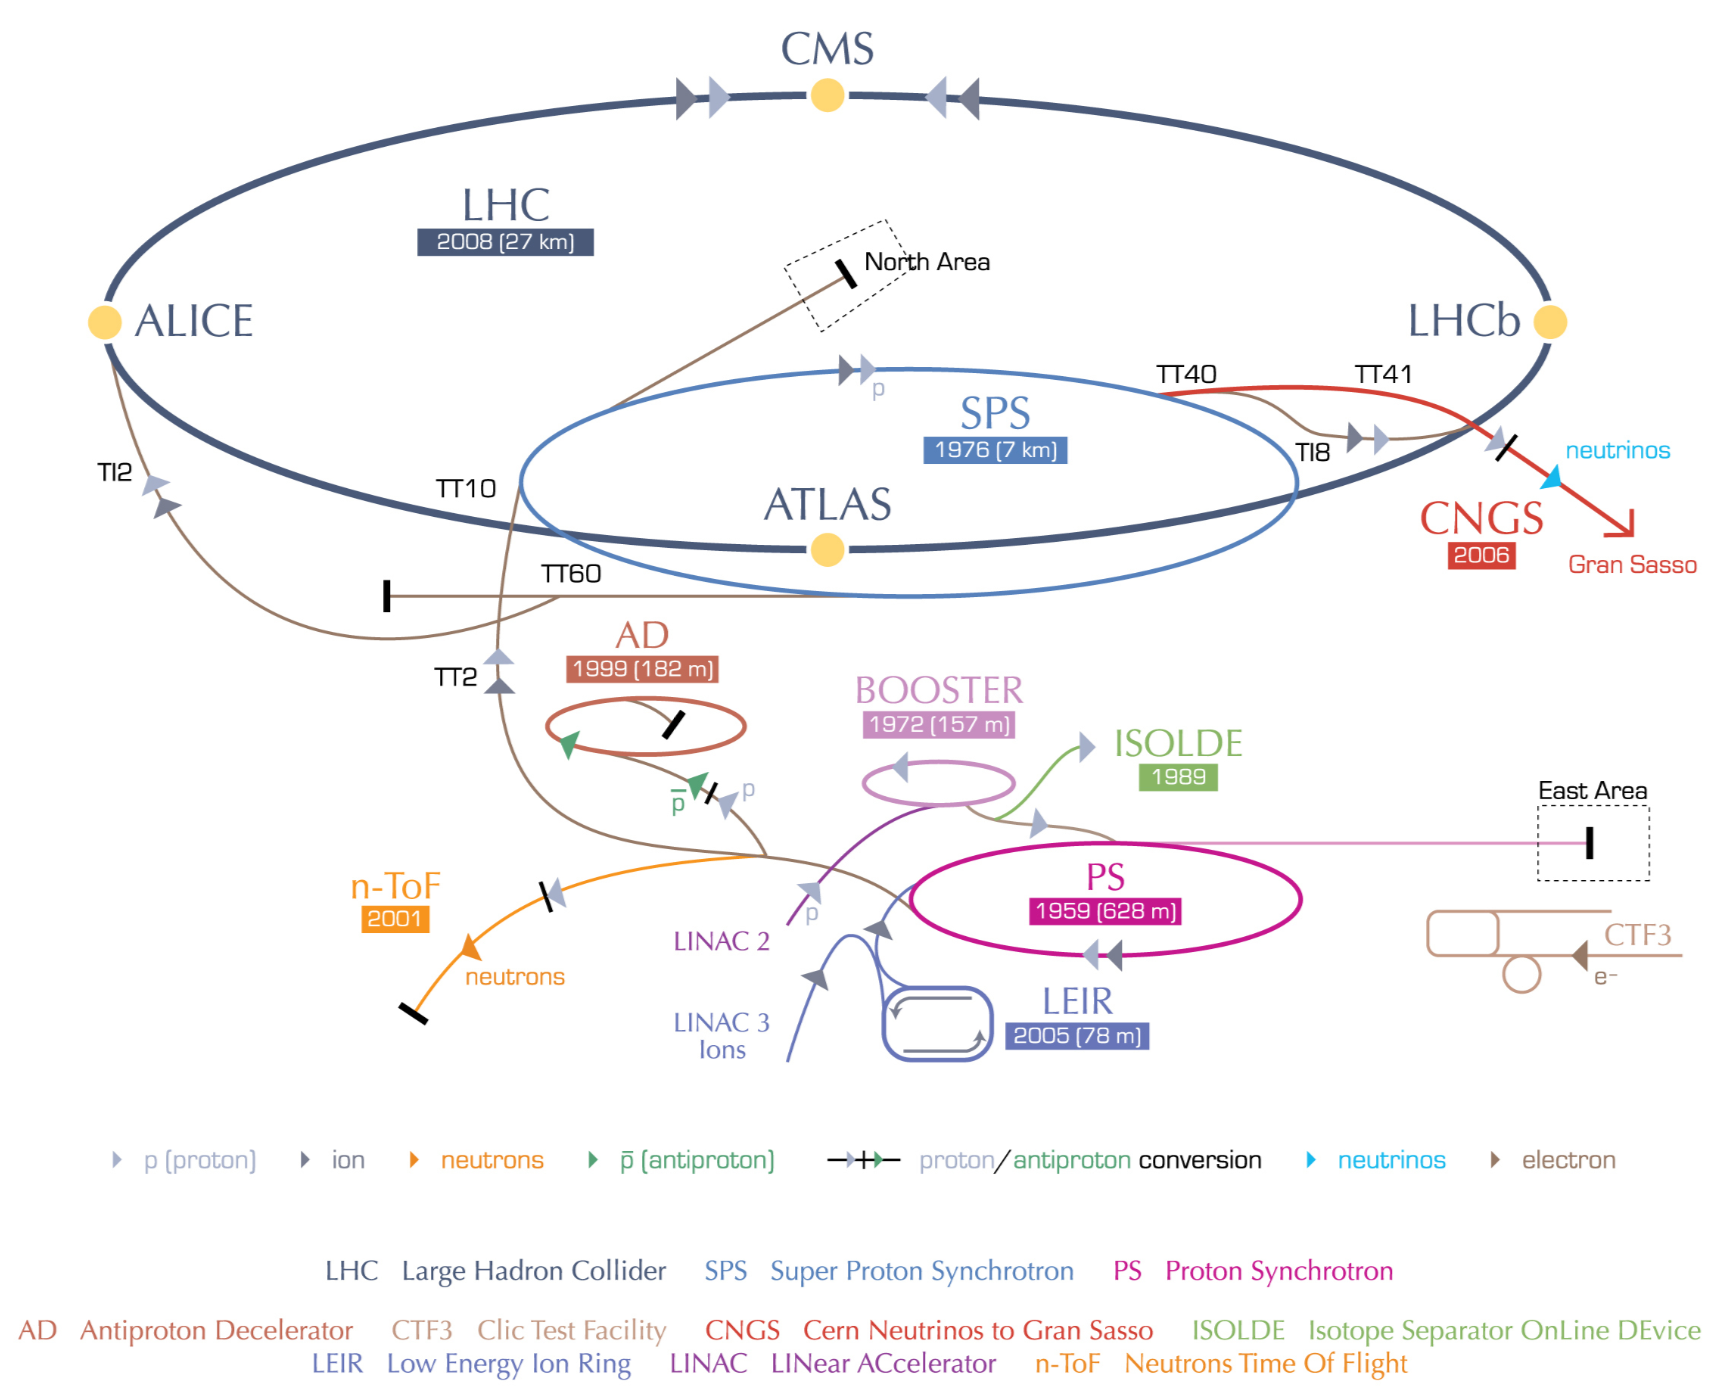
\includegraphics[width=0.8\textwidth]{gfx/lhc}
	\caption{Schematic view of the CERN accelerator complex and the LHC experiments~\cite{lhc}.}
	\label{fig:lhc}
\end{figure}

The protons injected in the LHC ring start their path in the LINAC2, where ionized hydrogen
atoms are accelerated up to 50 MeV. Then the beam is injected in the Proton Synchrotron Booster 
(PSB), which accelerates protons up to 1.4 GeV and provides the beam bunches to the Proton 
Synchrotron (PS). The Proton Synchrotron provides 25 GeV protons to the Super Proton Synchrotron
(SPS), where they are accelerated up to 450 GeV before the injection in the LHC.

Lead ions are produced from a highly isotopically pure $^{208}$Pb sample heated to a temperature
of about $800\,^{\circ}\mathrm{C}$.
The lead vapour is ionized by an electron current. Many different charge states are produced
with a maximum around Pb$^{29+}$.
These ions are selected and accelerated up to 4.2 MeV/u (energy per nucleon) before passing through
a carbon foil, which strips most of them to Pb$^{54+}$. The Pb$^{54+}$ beam is accumulated, then
accelerated to 72 MeV/u in the Low Energy Ion Ring (LEIR), which transfers them to the PS.
The PS accelerates the beam to 5.9 GeV/u and sends it to the SPS after the beam has passed through
a second foil where it is fully stripped to Pb$^{82+}$. 
The SPS accelerates the beam to 177 GeV/u and then the beam is sent to the LHC, which accelerates it
up to 5.02 TeV/u.

The LHC ring is composed by 1232 dipole magnets and 392 quadrupole magnets, which respectively 
guide and focus the counter–rotating beams in separate vacuum–filled pipes.
When the beams are stable they are brought into collision in four interaction points corresponding
to the experimental areas where the major LHC experiments are installed.
The top centre–of–mass energy reached at the LHC in the collisions are 13 TeV and 5.02 TeV per 
nucleon pair for pp and \pPb collisions, respectively.

Besides the centre–of–mass energy another crucial parameter for a collider is the luminosity
delivered to the experiments.
Indeed the number of events per second generated in the LHC collisions can be evaluated with the
following formula:
\begin{equation}
    R_{event} = L\;\sigma_{event}
\end{equation}
where $L$ is the machine instantaneous luminosity and $\sigma_{event}$ is the cross section for
the event under study. The instantaneous luminosity depends only on the beam parameters and can be 
written as:
\begin{equation}
    L = \frac{N_{b}N^{2} f_{rev} \gamma}{4\,\pi \epsilon_{n} \beta^{*}} F,
\end{equation}
where $N_{b}$ is the number of bunches in the collider ring, $N$ is the number of charges in each
bunch, $f_{rev}$ is the revolution frequency of the beam, $\gamma$ is the relativistic factor,
$\epsilon_{n}$ is the normalized emittance\footnote{$\epsilon_{n} = \beta \gamma \epsilon$ 
where $\beta$ and $\gamma$ are the usual relativistic factors and the emittance $\epsilon$ is the
spread of beam particles in the position-momentum phase space.} and $\beta^{*}$ is the value 
of the amplitude function\footnote{The amplitude function $\beta(s)$ describes the beam 
amplitude modulation due to the changing focusing strength.} at the interaction point (IP)
where the luminosity is estimated.

\begin{figure}
    \centering
    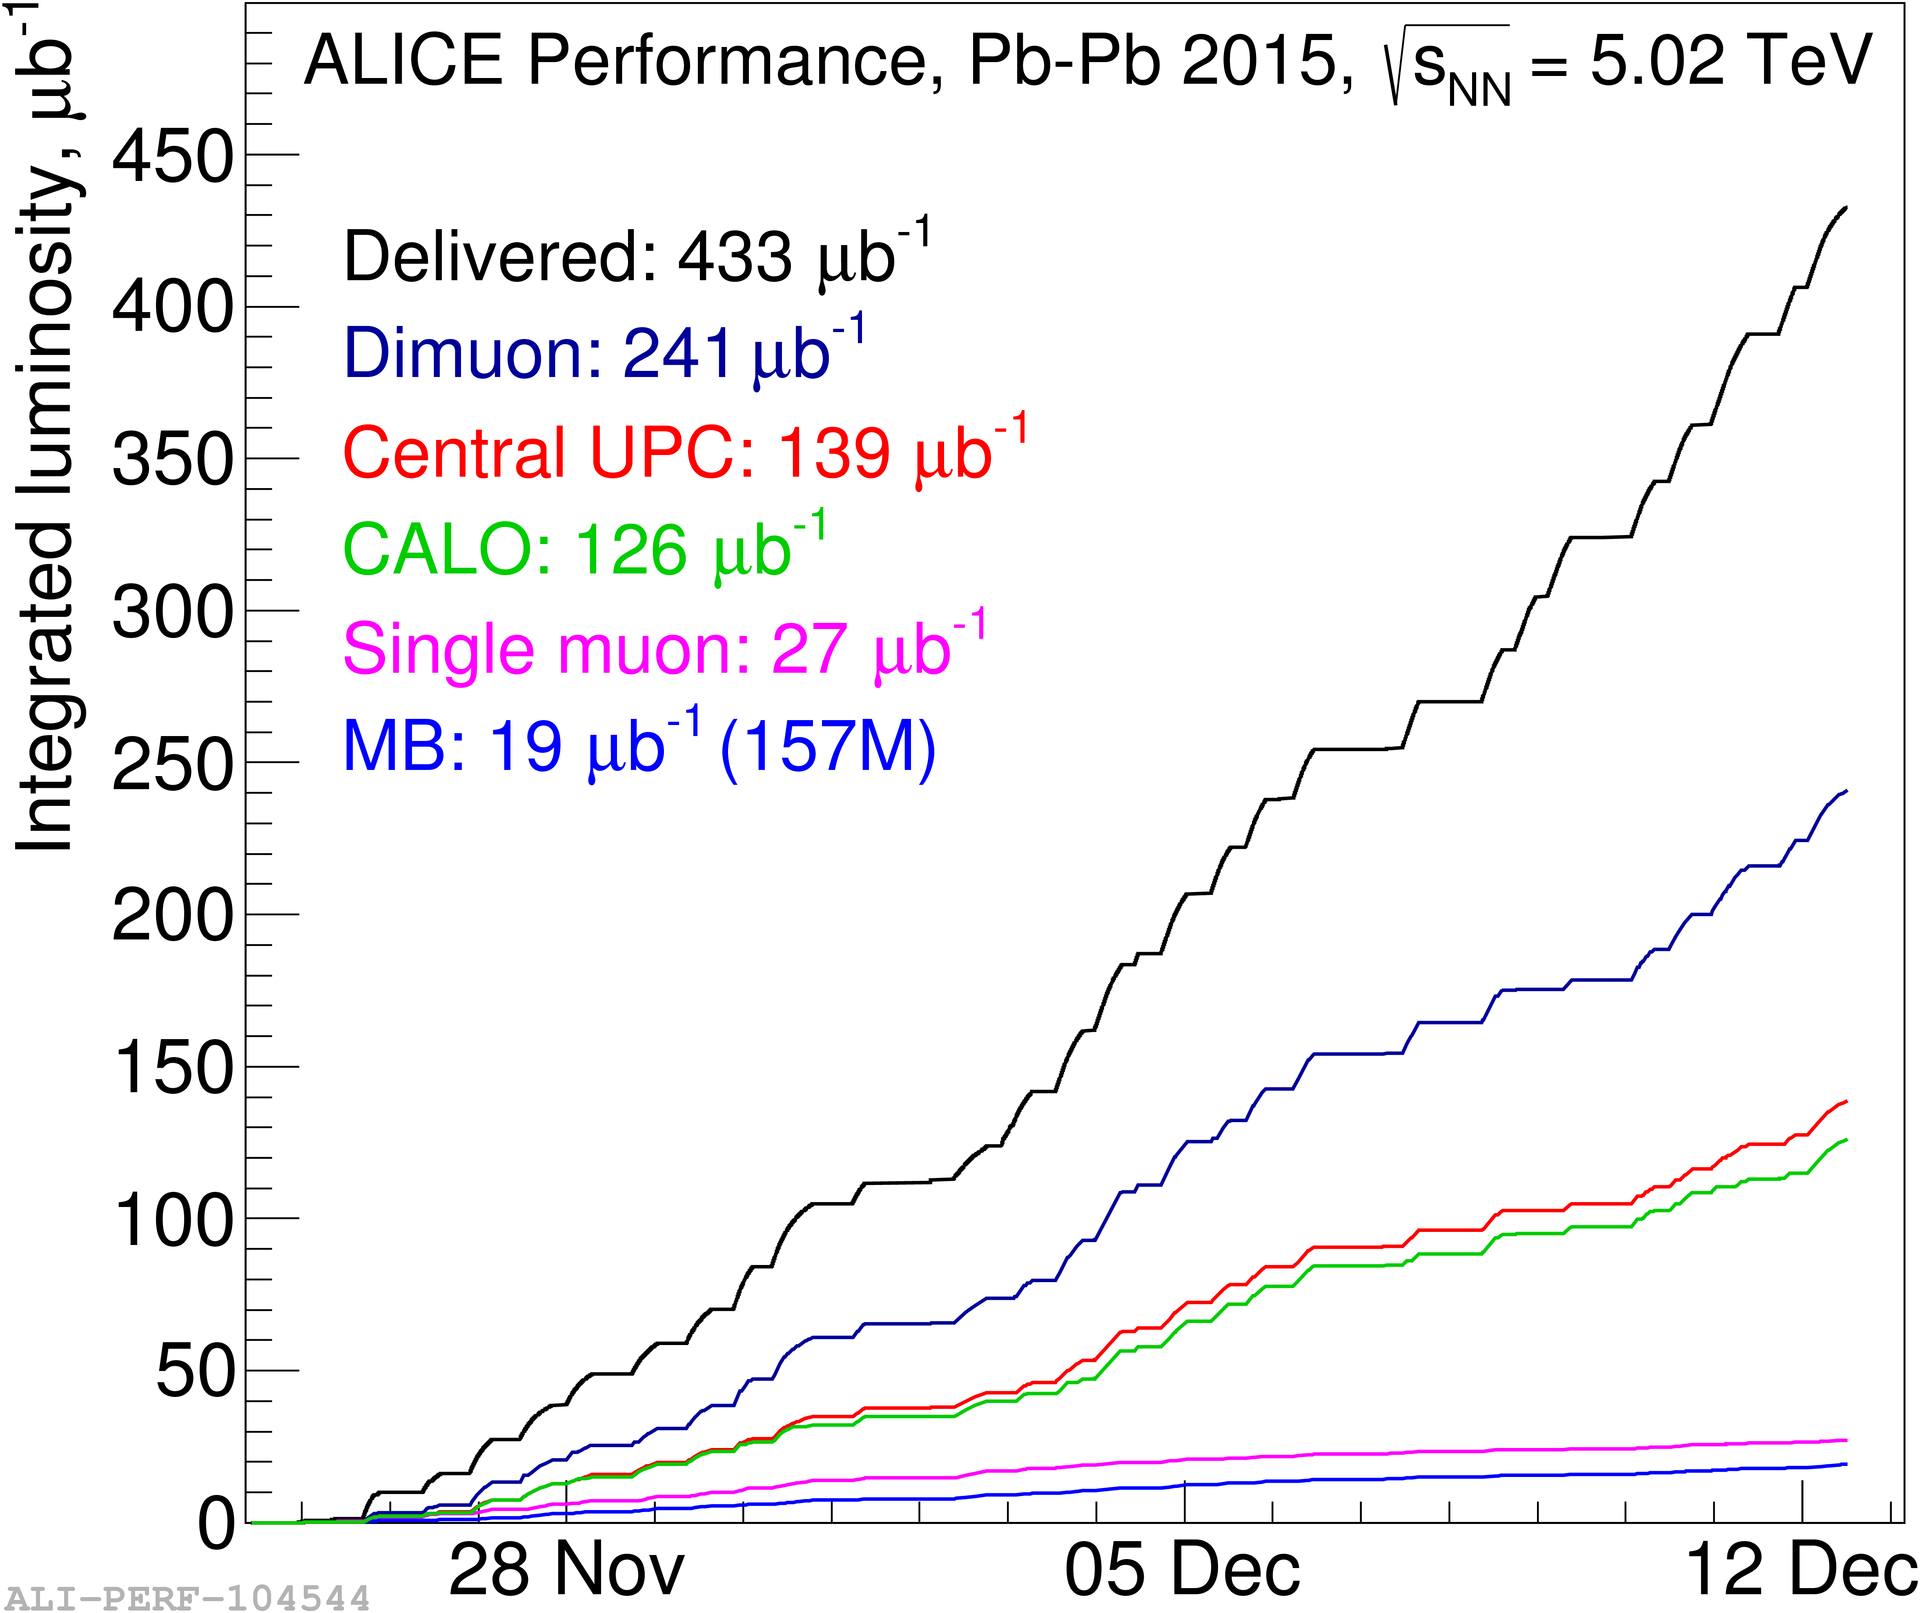
\includegraphics[width=0.6\textwidth]{gfx/alicelumi}
	\caption{ALICE delivered and integrated luminosity during the first Pb–Pb period in Run 2.}
	\label{fig:alicelumi}
\end{figure}

In order to maximise the luminosity of the LHC, the option of a p$\bar{\mathrm{p}}$ collider
was excluded due to the problem of the anti–protons production that is very complicated.
The LHC can store up to 2808 bunches, with $\sim 10^{11}$ protons per bunch, with 25 ns 
spacing~\cite{lhcperf}.
The ALICE apparatus requires a peak luminosity of $L = 10^{27}$ cm$^{-2}$s$^{-1}$ in \PbPb 
collisions.
Figure~\ref{fig:alicelumi} shows the delivered luminosity by the LHC (black line) and the integrated
luminosities collected by ALICE, for different trigger configurations (coloured lines), during the
first Pb–Pb period in Run 2 at the end of 2015.

A crucial information for the collider experiments is the position where the collision
between the two beams takes place: the \textit{primary vertex}. 
The nominal position of the primary vertex is the origin of the coordinate reference frame of the 
experiment. Nevertheless, due to the finite size of the bunches the position of the primary
vertex fluctuates around the nominal position.
Being $\sigma^{bunch}_{x,y,z}$ the \textit{rms} of the bunch in the transverse and longitudinal
direction, it can be shown that, assuming a gaussian profile of the bunches in the three directions,
the \textit{rms} of the vertex variation is:
\begin{equation}
    \sigma^{vertex}_{x,y,z} = \frac{\sigma^{bunch}_{x,y,z}}{\sqrt{2}},
\end{equation}
where the \textit{rms} size depends on the beam emittance and the amplitude function $\beta^{*}$:
\begin{equation}
    \sigma^{bunch}_{x,y,z} = \sqrt{\frac{\epsilon_{x,y,z}\,\beta^{*}}{\sqrt{\pi}}}.
\end{equation}
At the Interaction Point 2 (IP2), where the ALICE experiment is located, typical values for the vertex dispersion are 
$\sigma^{vertex}_{x,y}\,\sim 50\;\mu\mathrm{m}$ and $\sigma^{vertex}_{z}\,\sim 5\;\mathrm{cm}$.

%
%
\section{ALICE design} \label{sec:3.2}

The main goal of the ALICE experiment is the study of the QCD matter created in high energy heavy
ion collisions, hence the detector has been designed and optimised~\cite{alicedesign1,alicedesign2}
for this purpose.
A heavy ion experiment must have an efficient tracking system with a large acceptance and a good
particle identification (PID) capabilities in a wide momentum range, especially at low momentum.
Furthermore, it has to work in an environment characterized by a large charged particle multiplicity.
At the time of ALICE design, the charged particles multiplicity per rapidity unit in central Pb–Pb 
collisions was predicted to range between 2000 and 8000~\cite{alicemulti}, and for this reason
detectors with high granularity and low material budget have been 
developed~\cite{alicedesign1,alicedesign2}.

The current layout of the ALICE experiment is shown in Figure~\ref{fig:alice3D} while Table 
\ref{tab:alice} lists the position and the purpose of the ALICE sub-detectors.
\begin{figure}
    \centering
    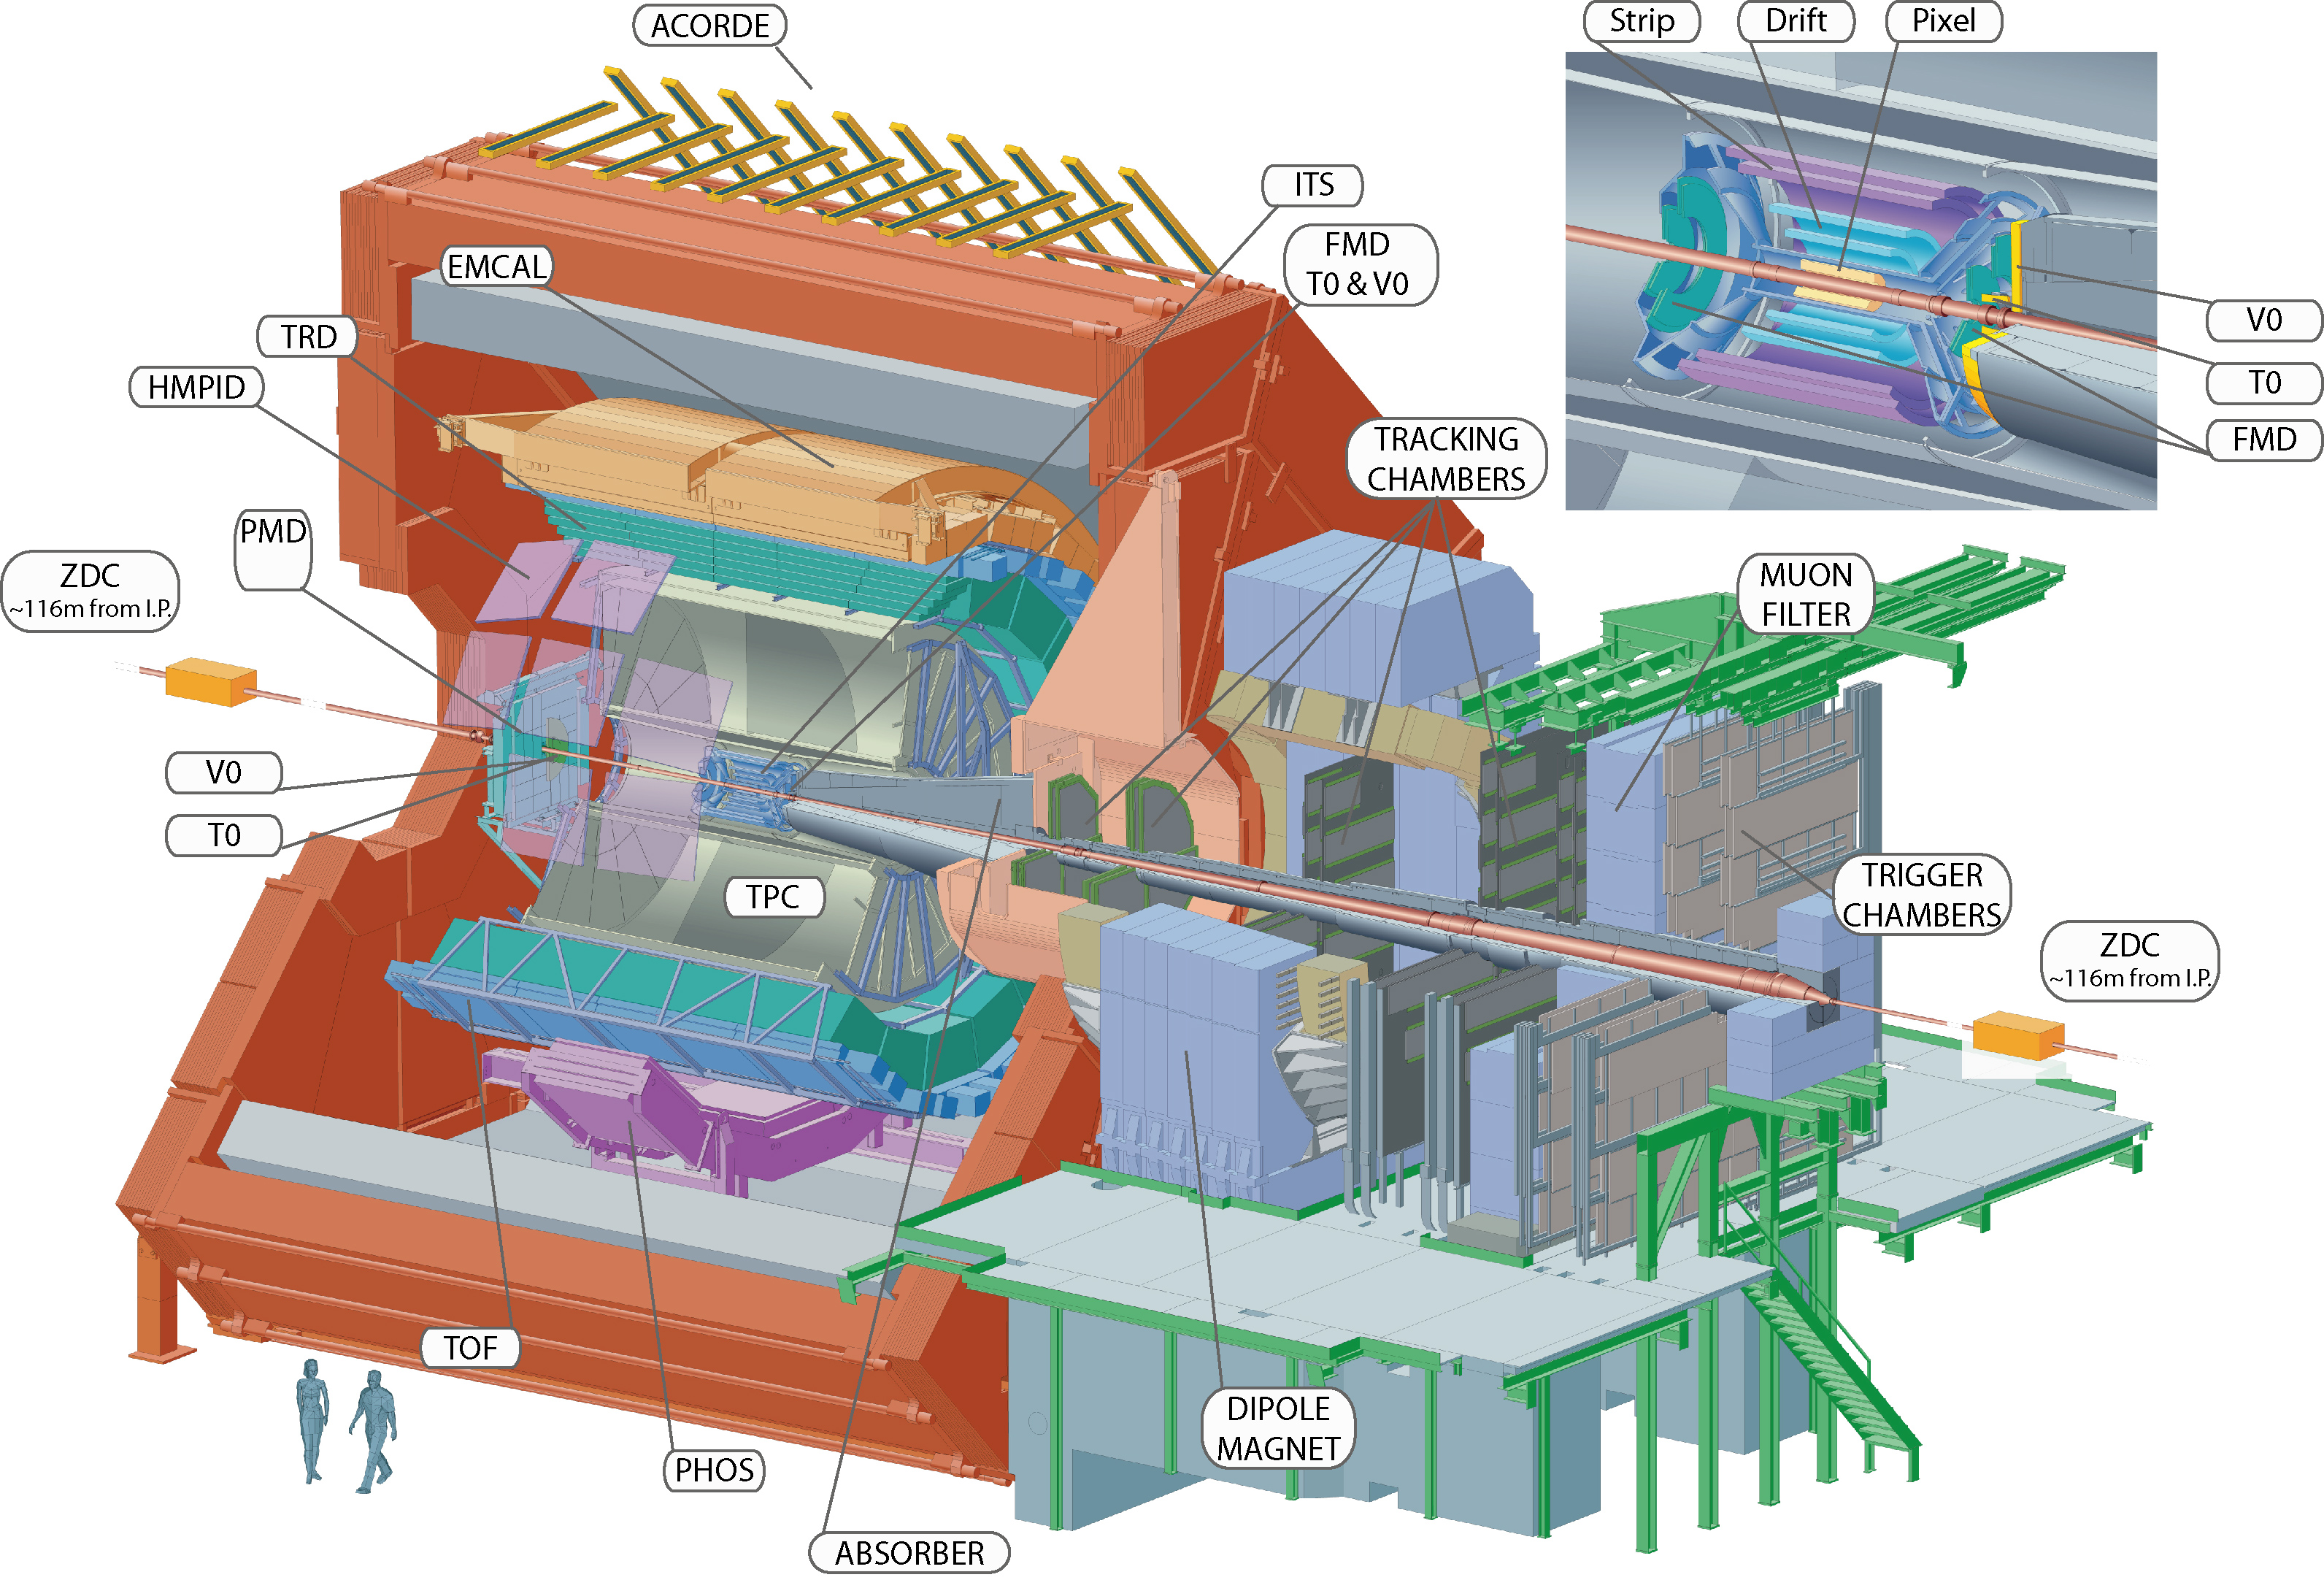
\includegraphics[width=0.9\textwidth]{gfx/alice3D}
	\caption{The ALICE experimental setup and the red L3 solenoid magnet. The top right inset shows a zoom on the V0, T0, FMD and the ITS detectors.}
	\label{fig:alice3D}
\end{figure}
The ALICE coordinate system is a right-handed orthogonal Cartesian system with the origin settled at
the nominal beams interaction point.
The $x$ axis is aligned with the horizontal accelerator plane and points to the centre of the LHC,
the $y$ axis is perpendicular to the accelerator plane and points upward.
As a consequence the $z$ axis is parallel to the beam direction and its positive direction is 
defined by the chirality of the coordinate system. 
For a more useful description of the apparatus and the physical quantities, two other coordinates
are defined, which together with the $z$ axis described above, form a cylindrical coordinate system:
the azimuthal angle $\phi$ increases counter-clockwise starting from $\phi = 0$ for $x$ axis looking
towards the Compact Muon Solenoid (CMS) side, and the polar angle $\theta$ increases from $z$ ($\theta=0$) to $-z$ 
($\theta=\pi$).
Other two useful variables, widely used in this thesis, are the \textit{pseudo-rapidity} $\eta$:
\begin{equation}
    \eta = \frac{1}{2} \ln \frac{|p| + p_{z}}{|p| - p_{z}} =
     - \ln \left[ \tan \left(\frac{\theta}{2} \right) \right],
\end{equation}
and the \textit{rapidity}:
\begin{equation} \label{eq:rapidity}
    y = \frac{1}{2} \log \bigl( \frac{E+p_{z}}{E-p_{z}} \bigr) 
\end{equation}
for a particle with four-momentum $p^{\mu} = (E,\vec{p})$, and the $z$ axis parallel to the beam 
direction.
For ultra-relativistic objects, the \textit{pseudo-rapidity} numerically converges to the 
\textit{rapidity}.

\begingroup
\setlength{\tabcolsep}{6pt} % Default value: 6pt
\renewcommand{\arraystretch}{1.2} % Default value: 1
\begin{table}[!tp]\small
\centering
	\begin{tabular*}{\textwidth}{@{\extracolsep{\fill}}lcccc}
	\toprule
		     & \multicolumn{2}{c}{\normalsize{\textbf{Acceptance}}} \\
	\textbf{\normalsize{Detector}} & \textit{\textbf{Polar}} & \textit{\textbf{Azimuthal}} & \textbf{\normalsize{Position}} & \textbf{\normalsize{Main purpose}}	 \\
    \midrule
	SPD$^{\dagger}$	\textit{layer 1}     & $|\eta|$ < 2.0	  & full			& r = 3.9 cm		& tracking, vertex\\
	SPD$^{\dagger}$	\textit{layer 2}     & $|\eta|$ < 1.4	  & full			& r = 7.6 cm		& tracking, vertex\\
	SDD	\textit{ layer 3}		         & $|\eta|$ < 0.9	  & full			& r = 15 cm		    & tracking, PID\\
	SDD	\textit{ layer 4}		         & $|\eta|$ < 0.9	  & full			& r = 23.9 cm	    & tracking, PID\\
    SSD	\textit{ layer 5}			     & $|\eta|$ < 1.0	  & full			& r = 38 cm		    & tracking, PID\\
    SSD	\textit{ layer 6}			     & $|\eta|$ < 1.0	  & full			& r = 43 cm		    & tracking, PID\\
    TPC	                                 & $|\eta|$ < 0.9     & full			& 85 < r/cm < 247   & tracking, PID \\
    TRD$^{\dagger}$	                     & $|\eta|$ < 0.8     & full			& 290 < r/cm < 368  & tracking, e$^{\pm}$ id \\
    TOF$^{\dagger}$	                     & $|\eta|$ < 0.9     & full			& 370 < r/cm < 399  & PID \\
    PHOS$^{\dagger}$                     & $|\eta|$ < 0.1    & 220$^{\circ}$<$\phi$<320$^{\circ}$	& 460 < r/cm < 478 & photons \\
    EMCal$^{\dagger}$                    & $|\eta|$ < 0.7     & 80$^{\circ}$<$\phi$<187$^{\circ}$	& 460 < r/cm < 478 & photons, jets \\
    HMPID                                & $|\eta|$ < 0.6     & 1$^{\circ}$<$\phi$<59$^{\circ}$		& r = 490 cm       & PID \\
    ACORDE$^{\dagger}$                   & $|\eta|$ < 1.3     & 30$^{\circ}$<$\phi$<150$^{\circ}$   & r = 850 cm       & cosmics \\
    \midrule
    PMD		                 & 2.3 < $\eta$ < 3.9   & full			& z = 367 cm		& photons\\
    FMD 	                 & 3.6 < $\eta$ < 5.0   & full			& z = 320 cm		& ch. particles\\
			                 & 1.7 < $\eta$ < 3.7	& full			& z = 80 cm		    & ch. particles\\
			                 & -3.4 < $\eta$ < -1.7 & full			& z = -70 cm		& ch. particles\\
	V0 A$^{\dagger}$         & 2.8 < $\eta$ < 5.1	& full			& z = 329 cm		& ch. particles\\
	V0 C$^{\dagger}$         & -3.7 < $\eta$ < -1.7	& full			& z = -88 cm		& ch. particles\\
	T0 A$^{\dagger}$         & 4.6 < $\eta$ < 4.9	& full			& z = 370 cm		& time, vertex\\
	T0 C$^{\dagger}$         & -3.3 < $\eta$ < -3.0	& full			& z = -70 cm		& time, vertex\\
	ZDC$^{\dagger}$		     & $|\eta|$ > 8.8	    & full			& z = $\pm$113 cm	& fwd neutrons\\
			                 & 6.5 < $\eta$ < 7.5	& $|\phi|$<10$^{\circ}$             & z = $\pm$113 cm	&fwd protons\\
			                 & 4.8 < $\eta$ < 5.7	& $|2\phi|$<32$^{\circ}$            & z = $\pm$113 cm   &photons\\
    \midrule
	MCH	                     & -4.0 < $\eta$ < -2.5 & full & -14.2 < z/m < -5.4  & muon tracking \\
	MTR$^{\dagger}$	         & -4.0 < $\eta$ < -2.5 & full & -17.1 < z/m < -16.1 & muon trigger \\	
    \bottomrule
    \end{tabular*}
    \vspace{2pt}
	\caption{Geometrical details and main purposes of the ALICE sub-detectors. This table has been taken and adapted from the description of the ALICE apparatus in~\cite{alice:Perf2014}. The transverse (r) and longitudinal ($z$) coordinates as well as the acceptance (\textit{polar} and \textit{azimuthal}) are measured with respect to the ALICE coordinate reference frame, described in the text. When more than one position value is specified the detector is divided in two or several parts and the reported values are the minimum and maximum distances from the interaction point. The detectors marked with a dagger ($\dagger$) are also used for triggering.}
	\label{tab:alice}
\end{table}
\endgroup

In the ALICE apparatus, three main parts can be distinguished: the \textit{central barrel}, the
\textit{muon spectrometer} and the \textit{forward detectors}.
In the following the main features of these parts are reported.
\paragraph{Central Barrel}
Consists of all the detectors located in the pseudo-rapidity range $|\eta| < 0.9$ and dipped in a 
solenoidal magnetic field (B = 0.5 T) produced by the warm resistive magnet previously used for
the L3 experiment at LEP~\cite{lep}.
The central barrel  tracking detectors include the Inner Tracking System (ITS), the Time Projection 
Chamber (TPC) and the Transition Radiation Detector (TRD), covering the full azimuthal acceptance.
These detectors, together with the Time Of Flight (TOF) detector and the High-Momentum 
Particle Identification (HMPID), provide also the information for particle identification (PID).
There are also an ElectroMagnetic Calorimeter (EMCal) and a Photon Spectrometer (PHOS) dedicated to the
physics of high \pt photons and jets.
Finally, on top of the ALICE solenoid, there is the ACORDE detector, an array of 60 large scintillators
used to study the high-energy cosmic air showers.

\paragraph{Muon Spectrometer} 
Located in the $-4 < \eta < -2.5$ region, is dedicated to the study of the spectrum of 
heavy-quark vector-mesons resonances.
It consists of an absorber wall with small atomic number Z, a spectrometer with a dipole magnet,
five tracking stations, four trigger stations and an iron absorber.

\paragraph{Forward Detectors}
Located in the forward-backward pseudorapidity regions and as close as possible to the beam line.
Forward detectors include: the Forward Multiplicity Detector (FMD) made of silicon strips detectors,
the Photon
Multiplicity Detector (PMD) and the Zero Degree Calorimeters (ZDC) consisting of two hadronic 
calorimeters for protons and neutrons, plus one electromagnetic calorimeter. 
In addition there are two trigger detectors located at each side of the interaction point:
the V0, made of scintillator detectors, and the T0, composed by two arrays of Cherenkov counters.

%
%
\section{ALICE detectors} \label{sec:alice_detectors}

In the following sections more details on the detectors used for the study of the \dst dibaryon
production are provided.

%
\subsection{Inner Tracking System} \label{sec:its}

The Inner Tracking System (ITS)~\cite{alicemulti,alice:Perf2014} is a silicon tracker and it is
the closest detector to the interaction point.
It is composed of six cylindrical layers of silicon detectors constructed by using three different
technologies.
In Figure~\ref{fig:its} the layout of the Inner Tracking System is shown, while in
Table~\ref{tab:its} more details on the resolution an the geometry of the different layers are
provided.

\begin{figure}
    \centering
    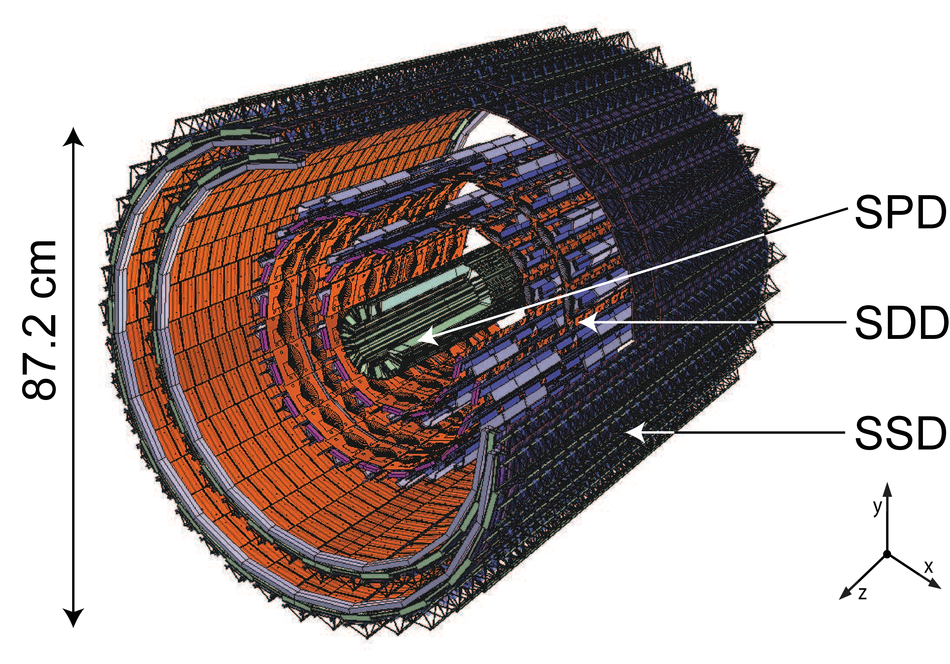
\includegraphics[width=0.7 \textwidth]{gfx/its}
	\caption{Layout of the ALICE Inner Tracking System, with three different subdetectors.}
	\label{fig:its}
\end{figure}

\paragraph{Silicon pixel detectors} 
SPD are the two innermost layers of the ITS and are
used for the determination of the primary vertex position as well as for the measurement of
the impact parameter of secondary tracks.
Furthermore, SPD, provides a quick trigger signal which contributes to the Level 0 trigger of 
the experiment.

\paragraph{Silicon drift detectors} 
SDD are the two intermediate layers of the ITS. The technology used for the SDD 
allows us to have high 2D resolution with limited number of read-out channels and to fulfil the
request of having a low material budget.

\paragraph{Silicon strip detectors}
SSD are the outer layers of the ITS and are equipped with double sided silicon detectors, which
provide a two dimensional measurement of the track position.
The information of the SSD is crucial for the matching of the tracks from ITS to TPC, being the
nearest layers to the TPC.

The main task of the ITS is the reconstruction of primary and secondary vertices, and the tracking
of the low \pt particles.
The first objective is achieved with a resolution better than 100 $\mu$m, while for the second the
ITS extends the tracking of the low \pt particles down to $\pt = 80 \; \mevc$, thanks to its high
spatial resolution (Tab.~\ref{tab:its}) and low material budget.
The total material budget of the ITS, keeping into account also the support structures and the 
thermal shields, is 7.18 \% X/X0.
The SSD, together with the SDD, provide also the measurement of the energy loss of particles 
in their sensitive volume, extending the ALICE Particle IDentification (PID) capabilities in the
 \pt region below 200 \mevc.

\begingroup
\renewcommand{\arraystretch}{1.2} % Default value: 1
\begin{table}
\centering
\begin{tabular}{lccc}
\textbf{Parameter}                      &  \textbf{SPD} & \textbf{SDD}  & \textbf{SSD} \\
\midrule
Material budget per layer (\%$X_{0}$)   &  1.14 - 1.14  &  1.13 - 1.26  &  0.83 - 0.86 \\
Spatial resolution $r\phi$ ($\mu$m)     &       12      &       35      &       20     \\
Spatial resolution $z$ ($\mu$m)         &       100     &       25      &      830     \\
Two track resolution $r\phi$ ($\mu$m)   &       100     &      200      &      300     \\
Two track resolution $z$ ($\mu$m)       &       850     &      600      &     2400     \\
Active cell size ($\mu$m$^2$)           & 50$\times$425 & 202$\times$294& 95$\times$40000 \\
Number of readout channels (k)          &      9835     &      133      &     2603     \\
\midrule
\end{tabular}
\vspace{2pt}
\caption{Details about the material budget and spatial resolution of the ITS subdetectors~\cite{alicemulti}. The material budget is reported for each single layer.}
\label{tab:its}
\end{table}
\endgroup

%
\subsection{Time Projection Chamber} \label{sec:tpc}

The Time Projection Chamber (TPC)~\cite{alice_tpc}, illustrated in Figure~\ref{fig:tpc}, 
is the main ALICE tracking detector with good two-track separation. 
It is also one of the main PID detectors as it provides the information about the specific energy 
loss of the particles in its volume in a large momentum range. 

\begin{figure} [!h]
    \captionsetup{justification=centering}
    \centering
    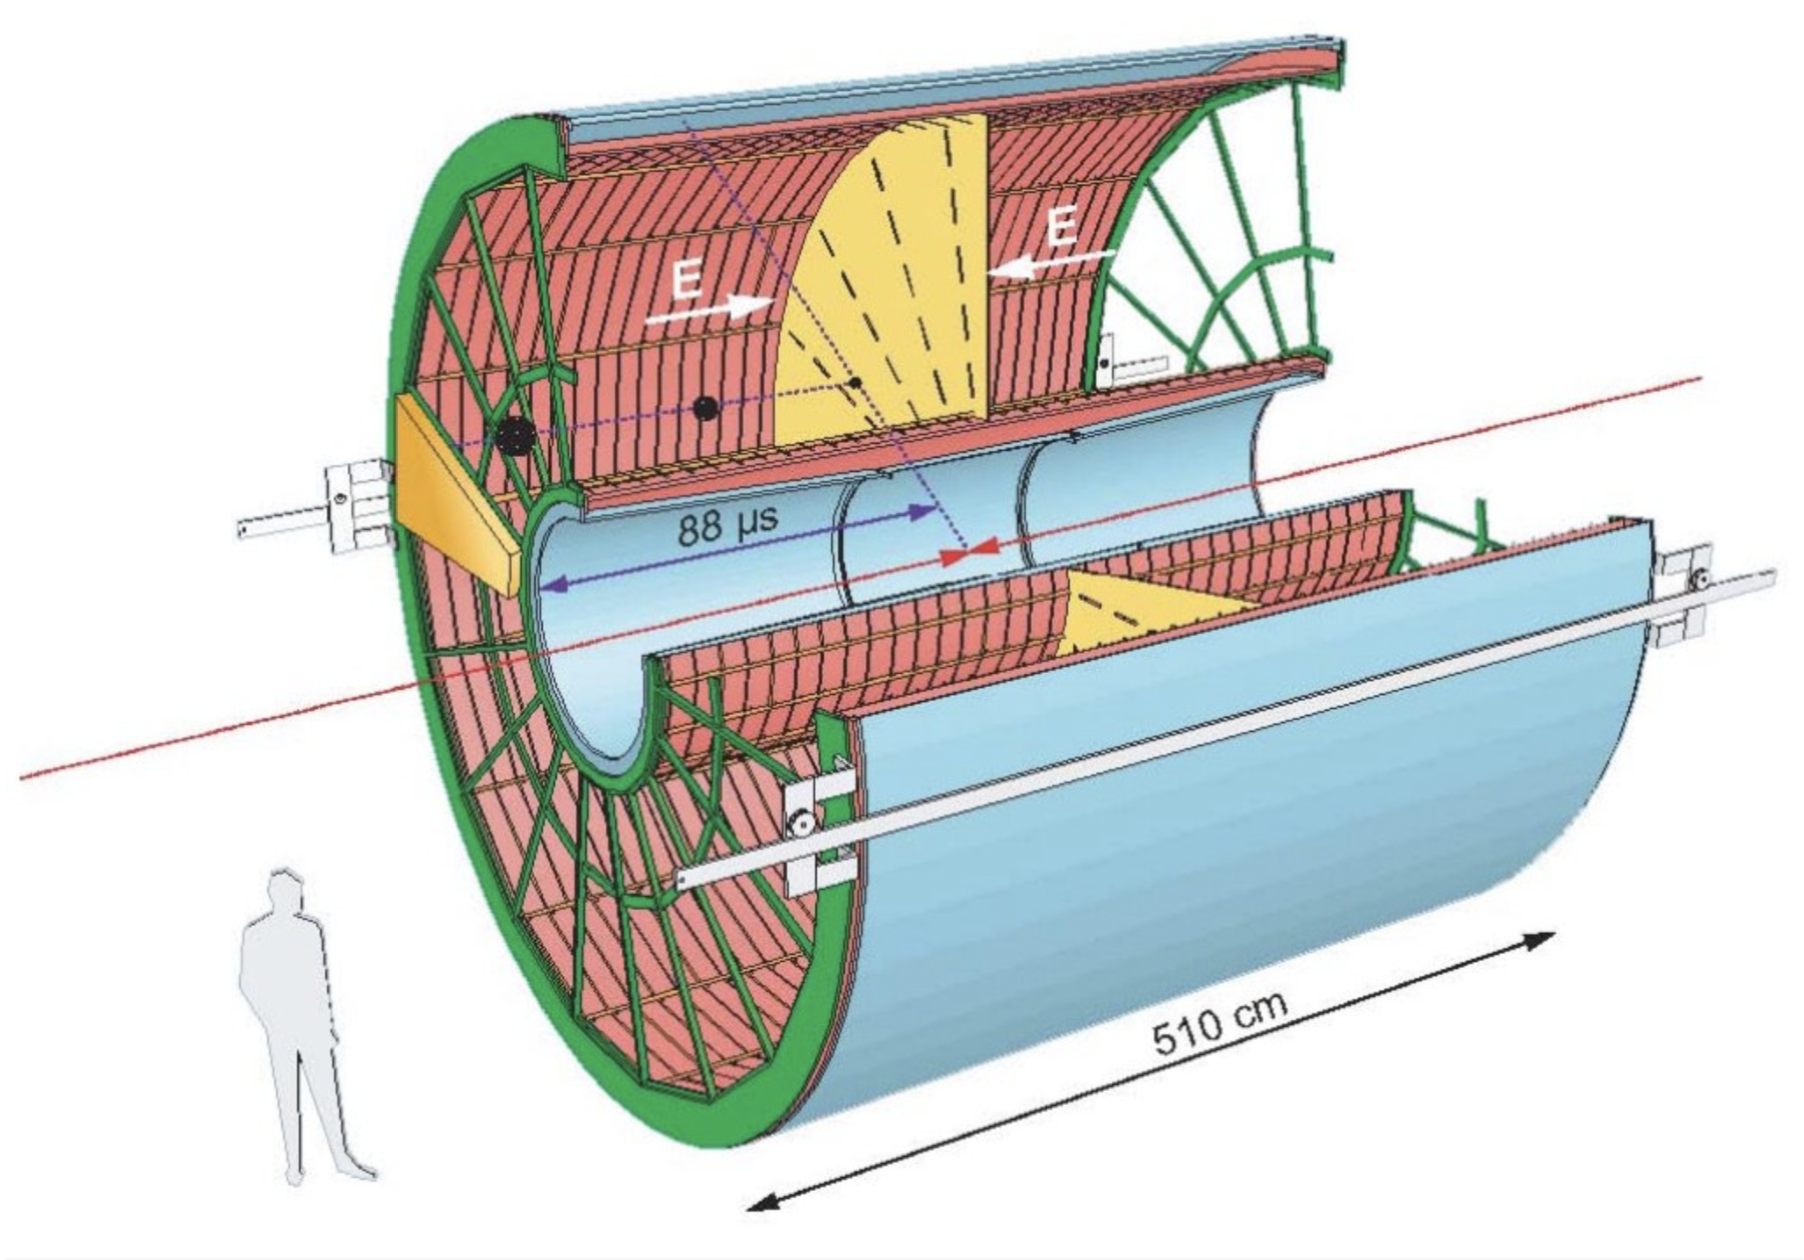
\includegraphics[width=0.8\textwidth]{gfx/tpc}
	\caption{Schematic layout of the ALICE Time Projection Chamber.}
	\label{fig:tpc}
\end{figure}

The TPC is a 88 m$^3$ cylinder filled with gas and divided in two drift regions by the
central electrode located at its axial centre. 
For the LHC Run 2 (2015-2018) the used gas is a mixture of Ar and CO$_2$.
The field cage secures the uniform electric field along the $z$ axis.
Charged particles travelling in the TPC gas ionise the gas along their path, liberating electrons 
that drift towards the end plates of the cylinder. 
Each end plate is equipped with 36 readout chambers, which are organized in 18 sectors, covering 
20$^{\circ}$ in azimuth each. 
The readout chambers consist in a system of multi-wire proportional chambers (MWPC) with cathode pad
read-out. Each sector is segmented by pads organized in rows and the longitudinal coordinate is given
by the drift time. 
Thanks to this segmentation, charged particles can be tracked and identified with up to 159 
3-dimensional space points (TPC clusters), including also the specific energy loss information
for the PID. The TPC radial position and acceptance are reported in Table~\ref{tab:alice}.

%
\subsection{Time Of Flight detector} \label{sec:tof}

The Time of Flight detector (TOF)~\cite{alice_tof} has a cylindrical geometry and consists of a 
large area array of Multi-gap Resistive-Plate Chambers (MRPC).
With a sensitive area of 7.4 × 120 cm$^2$ each and an intrinsic resolution of about $\sim\;$ 40
ps~\cite{alicemulti}.
TOF is used to identify charged particles and light nuclei in the momentum interval 
0.2--4 \gevc in the central pseudorapidity range ($|\eta|$ < 0.9).
The time of flight of a particle is determined by measuring the time between the event collision and
the particle TOF hit cluster. 
The time of flight of the particle together with the momentum, obtained from the track curvature, 
allows us to compute the particle $\beta$ and, as a consequence, its mass.
The precise determination of the event collision time, the so called $t_{0}$, represents an important
ingredient for the TOF PID and it is determined by using the information from the T0 detector as 
well as from the TOF. 

%
\subsection{T0 detector} \label{sec:t0}

The T0 detector~\cite{alice_t0} consists of two arrays of Cherenkov counters placed on both 
sides of the interaction point along the $z$ axis (Tab.~\ref{tab:alice}).
It is mainly used to determine the event collision time ($t_{0}$) with a resolution below 50 ps
and  independently from track and vertex reconstruction. 
The T0 information provides also the Level 0 trigger when the position of the vertex falls in
appropriate intervals.

%
\subsection{V0 detector} \label{sec:v0}

The V0~\cite{alice_v0} is a small angle detector consisting of two arrays (V0A and V0C) of 64 
scintillators counters distributed in 8 rings and they are installed on both sides of the ALICE
interaction point (Tab.~\ref{tab:alice}). 
The V0 detectors are used to define the minimum bias (MB) trigger in ALICE and to determine the
centrality in \pPb and \PbPb collisions.

%
%
\section{Trigger and Data Acquisition} \label{sec:data_flow}

The trigger system in ALICE is managed by the Central Trigger Processor (CTP)~\cite{alice_trigger} 
which collects and synchronises all the trigger inputs coming from all the triggering detectors 
with the information on the LHC filling scheme providing a trigger signal to the readout detectors
in case of fulfilled trigger conditions. 
The Level 0 trigger (L0) decision is taken by using the fast detectors: SPD, V0, T0, EMCal, PHOS and 
muon trigger. The L0 signal arrives to the CTP in 1.2 $\mu$s after the collision happens. 
The signals from the detectors which are not fast enough for L0 trigger are collected in the level 1
(L1) trigger signal and sent to the CTP after 6.5 $\mu$s. 
Finally the third level trigger is sent after 88 $\mu$s, which is the maximum drift time of electrons
in the TPC, in order to maximize the rejection of the pile-up events in the TPC.
The minimum-bias (MB) trigger  selection in ALICE is defined by the logical "\textit{or}" between the
signals of V0A, V0C and SPD detectors. This minimum-bias trigger is the one used in the analysis
presented in this thesis.

The events passing all three trigger selections are then sent to both the Data Acquisition (DAQ) machines 
and to the High Level Trigger (HLT).


The data fulfilling all the trigger requirements, are sent to the Local Data Concentrators (LDCs)
through optical connections, the Detector Data Links (DDLs).
LDCs is a farm of computers which build \textit{subevents} from the event fragments they receive from
the front-end electronics and then sends \textit{subevents} to the Global Data Collectors (GDCs).
The GDC compose the full event including information from the HLT.
At the HLT level a fast reconstruction of the data \ -- including clusterisation and track
reconstruction -- \ is performed, allowing further selections that are not possible in the hardware
triggers.
When the event building in the GDC is completed, the data are buffered in a local disk pool waiting 
to be transferred to the CERN computing centre, where they will be registered on tape.

%
%
\section{ALICE offline framework} \label{sec:offline}

The offline analysis framework is fundamental for any High Energy Physics experiment.
The huge amount of data collected by detectors requires a proper infrastructure able to process and 
analyse the reconstructed events.
Beyond that, modern experiments need a large number of Monte Carlo (MC) simulations, for the
development of the detectors, for performance studies, and also as a basis for physics analyses.

The infrastructure realised at CERN in order to menage the LHC data flow is the Worldwide 
LHC Computing Grid (WLCG). The mission of this project is to provide global 
computin3 resources to store, distribute and analyse the $\sim$50-70 Petabytes of data expected for 
each year of operations of the LHC experiments.

The ALICE collaboration uses the WLCG resources for running MC simulations, event reconstruction and
physics analyses. 
In the following section more details about this aspects of the ALICE operations will be provided.

%
\subsection{Monte Carlo simulations} \label{sec:montecarlo}

The first step of Monte-Carlo simulations is the event generation. 
The ALICE simulation tools include generators suited for the different collision systems available at
the LHC: proton-proton (pp), proton-ion (pA) and heavy ion (AA) collisions.
The event generator gives the set of all stable and weakly decaying particles produced in the
collision, with their starting kinematic parameters. 
The strongly decaying particles -- as the \dst dibaryon studied in this analysis -- are usually 
handled at the generator level.
Then, the generated kinematic parameters are propagated, using a transport code, through the
experiment, whose geometry and material budget are precisely described in the ALICE software.

Three different transport codes are available in the simulation framework: GEANT3~\cite{geant3},
GEANT4~\cite{geant4}, and FLUKA~\cite{fluka1,fluka2}.
These tools provide the information on the behaviour of the transported particles through the sensitive
part of the detector, giving the particle energy loss. 
This information is then converted in detectors electronics signal through the simulation of each
detector response.
Finally, the digitalised signal is stored in the same detector raw data format used in the 
real data taking and reconstruction.

%
\subsection{Event Reconstruction} \label{sec:event_rec}

The ALICE event reconstruction flow starts from the raw data, collected or simulated, and its flow is 
schematically shown in Figure~\ref{fig:rec_flow}. 

In the first step of the event reconstruction the detector raw data are converted into clusters, 
through a set of algorithms which perform the reconstruction for each detector separately.
All clusters are characterized by positions, signal amplitude and time.
Other information, like the energy lost by the particle, the time of flight or the Cherenkov 
angle are attached to the clusters in the PID detectors allowing the identification of the 
tracked particle.

The second step of the reconstruction is a preliminary estimation of the position of the primary
vertex using clusters in the SPD, the closest detectors to the interaction point.
The first estimate of the primary vertex is fundamental to speed-up the tracking algorithm in the 
phase dedicated to the search of good candidate tracks, even if the final estimation of the 
interaction vertex position needs the full track information.

Subsequently, the Kalman filter technique~\cite{kalman} is used to perform track finding and
fitting in the TPC and the ITS. 
The main tracking detector, in ALICE, is the Time Projection Chamber and therefore tracks are 
reconstructed  starting from the TPC, then they are prolonged in the ITS looking for matches with
the ITS reconstructed tracks. 
The found tracks are backward propagated searching, also, for a possible match in the other central
barrel detectors.
Finally, the primary vertex can be determined using the fully reconstructed tracks.

The last step of the event reconstruction chain is the search for photon conversion and decays of
strange hadrons.

\begin{figure}
    \captionsetup{justification=centering}
    \centering
    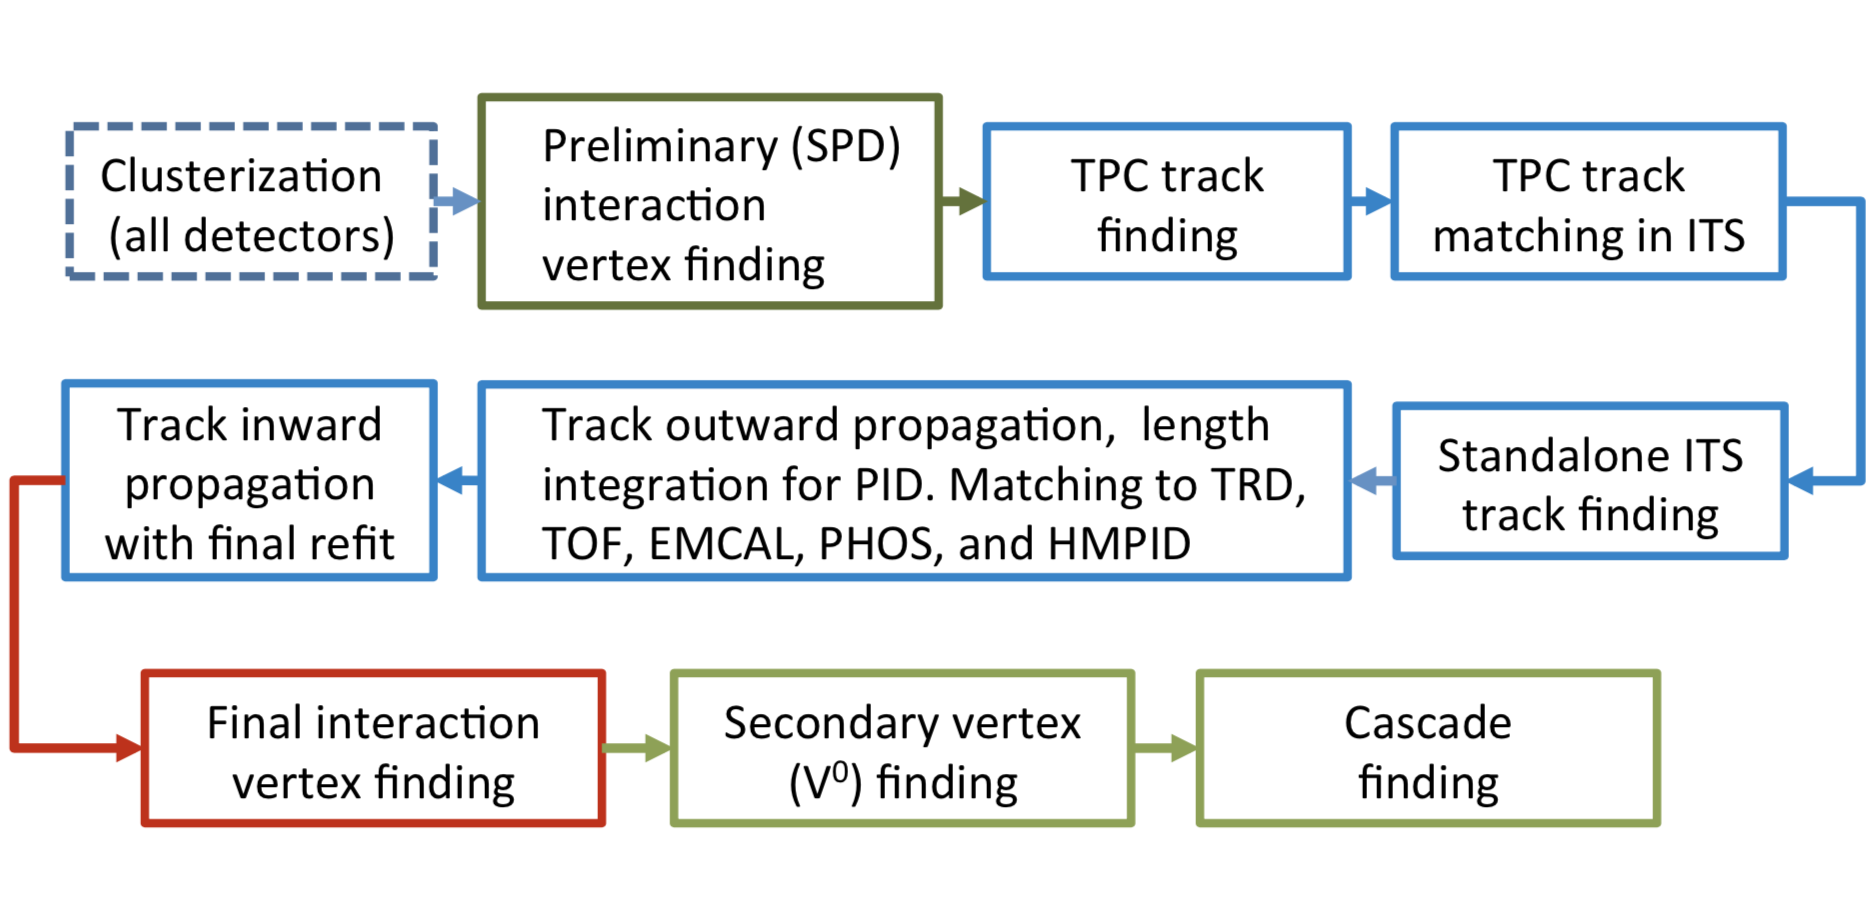
\includegraphics[width=0.9\textwidth]{gfx/reconstruction}
	\caption{Vertex and tracks reconstruction procedure in ALICE \cite{alice:Perf2014}.}
	\label{fig:rec_flow}
\end{figure}

%
\subsection{ALICE analysis framework} \label{sec:anal_frame}

The ALICE software infrastructure that allows the whole Collaboration to access the collected and
simulated data on the grid, is the Alien (ALICE Environment)~\cite{alien} grid middleware.
Through the Alien user interface it is possible to launch the analysis tasks on ALICE data. 
When more users are interested in analyzing the same data sample, one can use an optimized
access pattern, called \textit{analysis train}, which allows to run together all the tasks
of those users in the same job.
This procedure defines a standard analysis flow in the ALICE experiment and it ensures the
reproducibility of the analyses.

The data collected by the ALICE experiment are stored in binary files using the ROOT framework data 
format.
The ALICE software environment, called \textit{AliRoot}, was introduced in 1998 and it is based on 
the ROOT framework~\cite{root}.
The analysis related code -- containing all the software used in physics analyses -- is collected
in a part of the ALICE offline framework denominated \textit{AliPhysics}.
The reconstructed events are stored in two different formats: the Event Summary Data (ESD) format, 
that is mainly used for calibration and detector performance studies, and the Analysis Object Data 
(AOD) format, which contains only the relevant information at the analysis level.

%
%
\section{ALICE performances} \label{sec:ali_perf}

The ALICE experiment was specifically designed for the demanding experimental environment created in 
\PbPb collisions. 
One of the most challenging task, in these conditions, is the precise reconstruction of both momentum
and origin of the produced particles.
In this section the tracking and vertexing performances of the ALICE experiment will be presented,
as well as the methods used for the particle identification.

%
\subsection{Tracking} \label{sec:tarcking}

The importance of the tracking process lies in its relation with the particle momentum
measurement and with the vertexing determination (Sec.~\ref{sec:vertexing}).

The momentum of a charged particle travelling in a magnetic field is related to the radius of curvature
of the particle track. Therefore, by measuring the radius of curvature, one can determine the
particle momentum.
In particular, in collider experiments, the interaction point is surrounded by cylindrical 
position-sensitive detectors located in magnetic field -- usually parallel to the beam axis -- 
which provide a measurement of the \textit{sagitta} of the track.
The particle momentum is related to the sagitta $s$ by the following expression:
\begin{equation}
    p = \frac{L^{2} q B}{8\,s},
\end{equation}
where $L$ is the lever arm length of the tracking detectors, $q$ is the charge of the particle and $B$
the magnetic field.
Therefore, the resolution on the particle momentum does not depend only on the magnetic field,
but also on $L$ and, of course, on the resolution on the sagitta $\sigma_{s}$:
\begin{equation}
    \frac{\sigma_{p}}{p} \propto p \frac{\sigma_{s}}{B\,L^{2}}.
\end{equation}
Thanks to the large radial coverage ($0.039 \leq r \leq 3.680\ $ m), despite the mild solenoidal
magnetic field, the ALICE apparatus is able to reconstruct tracks over a wide momentum range.

The first stage of the tracking algorithm starts building the track seeds at a large radius of 
the TPC.
The seeds are propagated inward looking for other TPC clusters compatible with the track.
Whenever a compatible cluster is found, the track parameters are updated using a Kalman 
filter~\cite{kalman}. 
Different seeds can reuse the same cluster, therefore it is not uncommon to have two or more
tracks sharing some clusters. 
If the fraction of shared clusters is above a predefined threshold (between 25\% and 50\%), a
dedicated algorithm rejects the candidate tracks with the worst quality parameters.
The tracks with at least 20 clusters (out of a maximum of 159) and that miss no more than 50\% 
of the expected clusters are accepted and propagated to the inner radius of the TPC.
Figure~\ref{fig:reconstruction} shows the track reconstruction efficiency of the TPC.

\begin{figure}
    \centering
    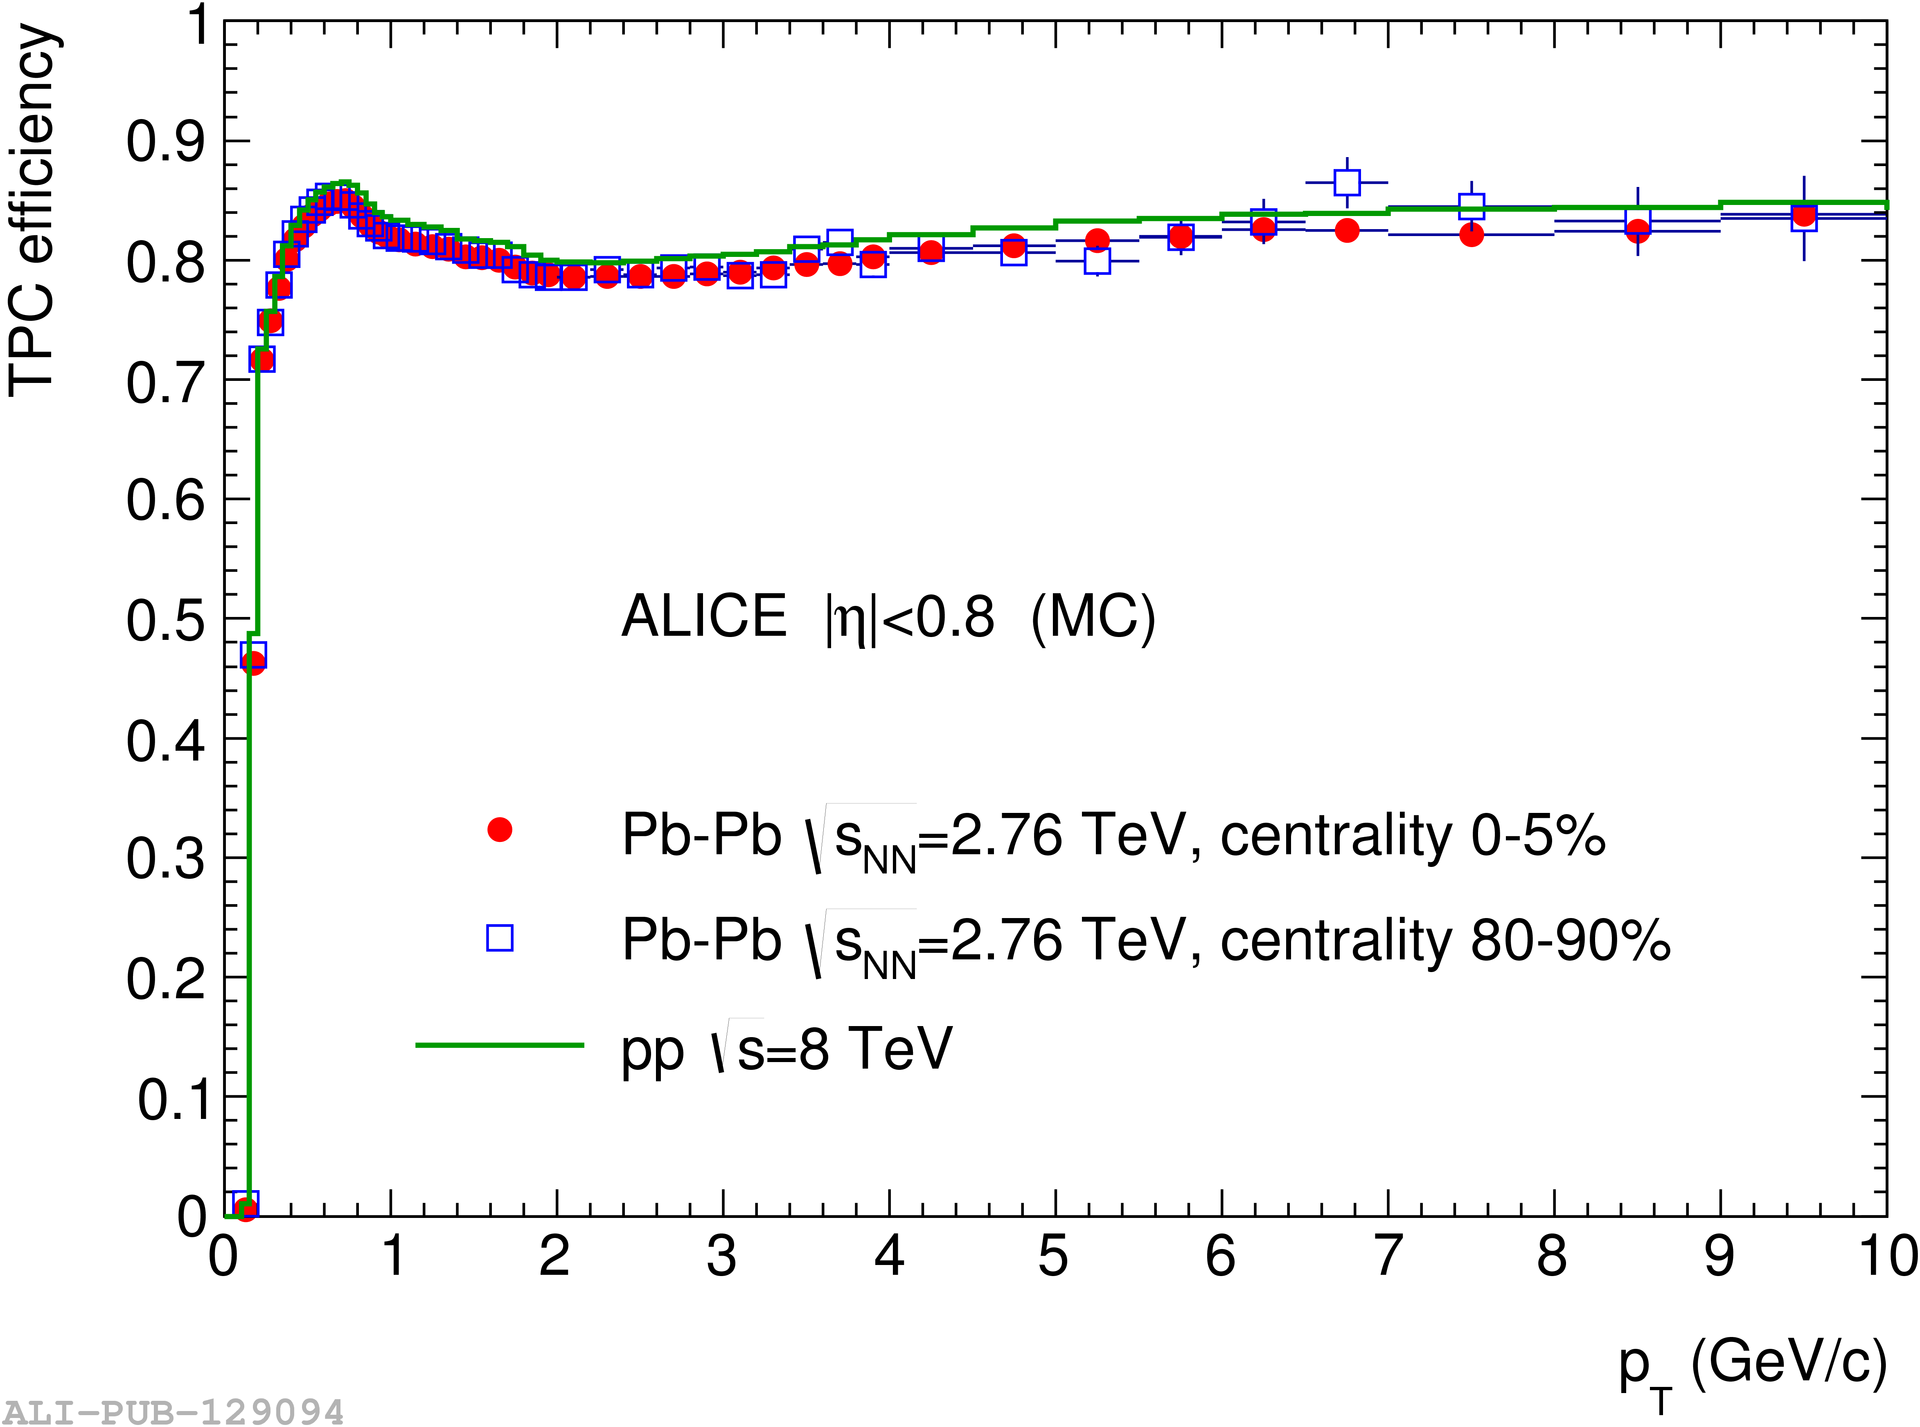
\includegraphics[width=0.7\textwidth]{gfx/tpc_rec_eff}
	\caption{TPC track reconstruction efficiency in pp (green line) collisions at \sotev and for central (red dots) and peripheral (blue open square) \PbPb collisions at \sdtev. The drop for $\pt \leq 0.5\; \gevc$ is due to energy loss in the detector material and the shape at higher \pt is related to the loss of clusters in the dead zones of the TPC. The efficiency does not depend on the detector occupancy.}
	\label{fig:reconstruction}
\end{figure}

The reconstructed TPC tracks are then propagated to the SSD, the outermost layer of the ITS.
At this point, the tracking algorithm in ITS proceeds with a procedure similar to that adopted
for the TPC. 
Starting from the second layer of SSD, the seeds are propagated inward, penalizing tracks
for which a compatible cluster in the extrapolation is not found.
Among the prolongation candidates of the TPC track only the highest quality track candidate is
selected. This track is finally stored in the reconstructed event as ITS+TPC track.

The second stage of the tracking algorithm is the backward refit of the ITS+TPC tracks performed by
using the Kalman filter.
The track is backward propagated looking for matching with TRD tracklets. If the matching is
successful, the algorithm updates the track parameters using the TRD tracklet information. 
During this process, at each step, the integrated track length and the expected time of flight
for different particle species are computed and the related track parameters are updated.
This information is used for a correct particle identification in the Time Of Flight detector
(Sec.~\ref{sec:PID}).
Then an attempt to extrapolate the track and match it to one of the TOF clusters is performed.
The track length integration and time of flight calculation are stopped at this stage.
Finally a further extrapolation is performed to match the track with other external central
barrel detectors as HMPID, PHOS and EMCal.

The final stage of the track reconstruction, consists in propagating all the tracks from the TRD
back to the innermost ITS layer. 
In each detector (TRD, TPC and ITS) the tracks are refitted by using the information of all attached
clusters.
If the refit process goes well the track \textit{refit flag} is switched on.
At this stage the track’s position, direction, inverse curvature and its associate covariance 
matrix are determined.

\begin{figure}
    \centering
    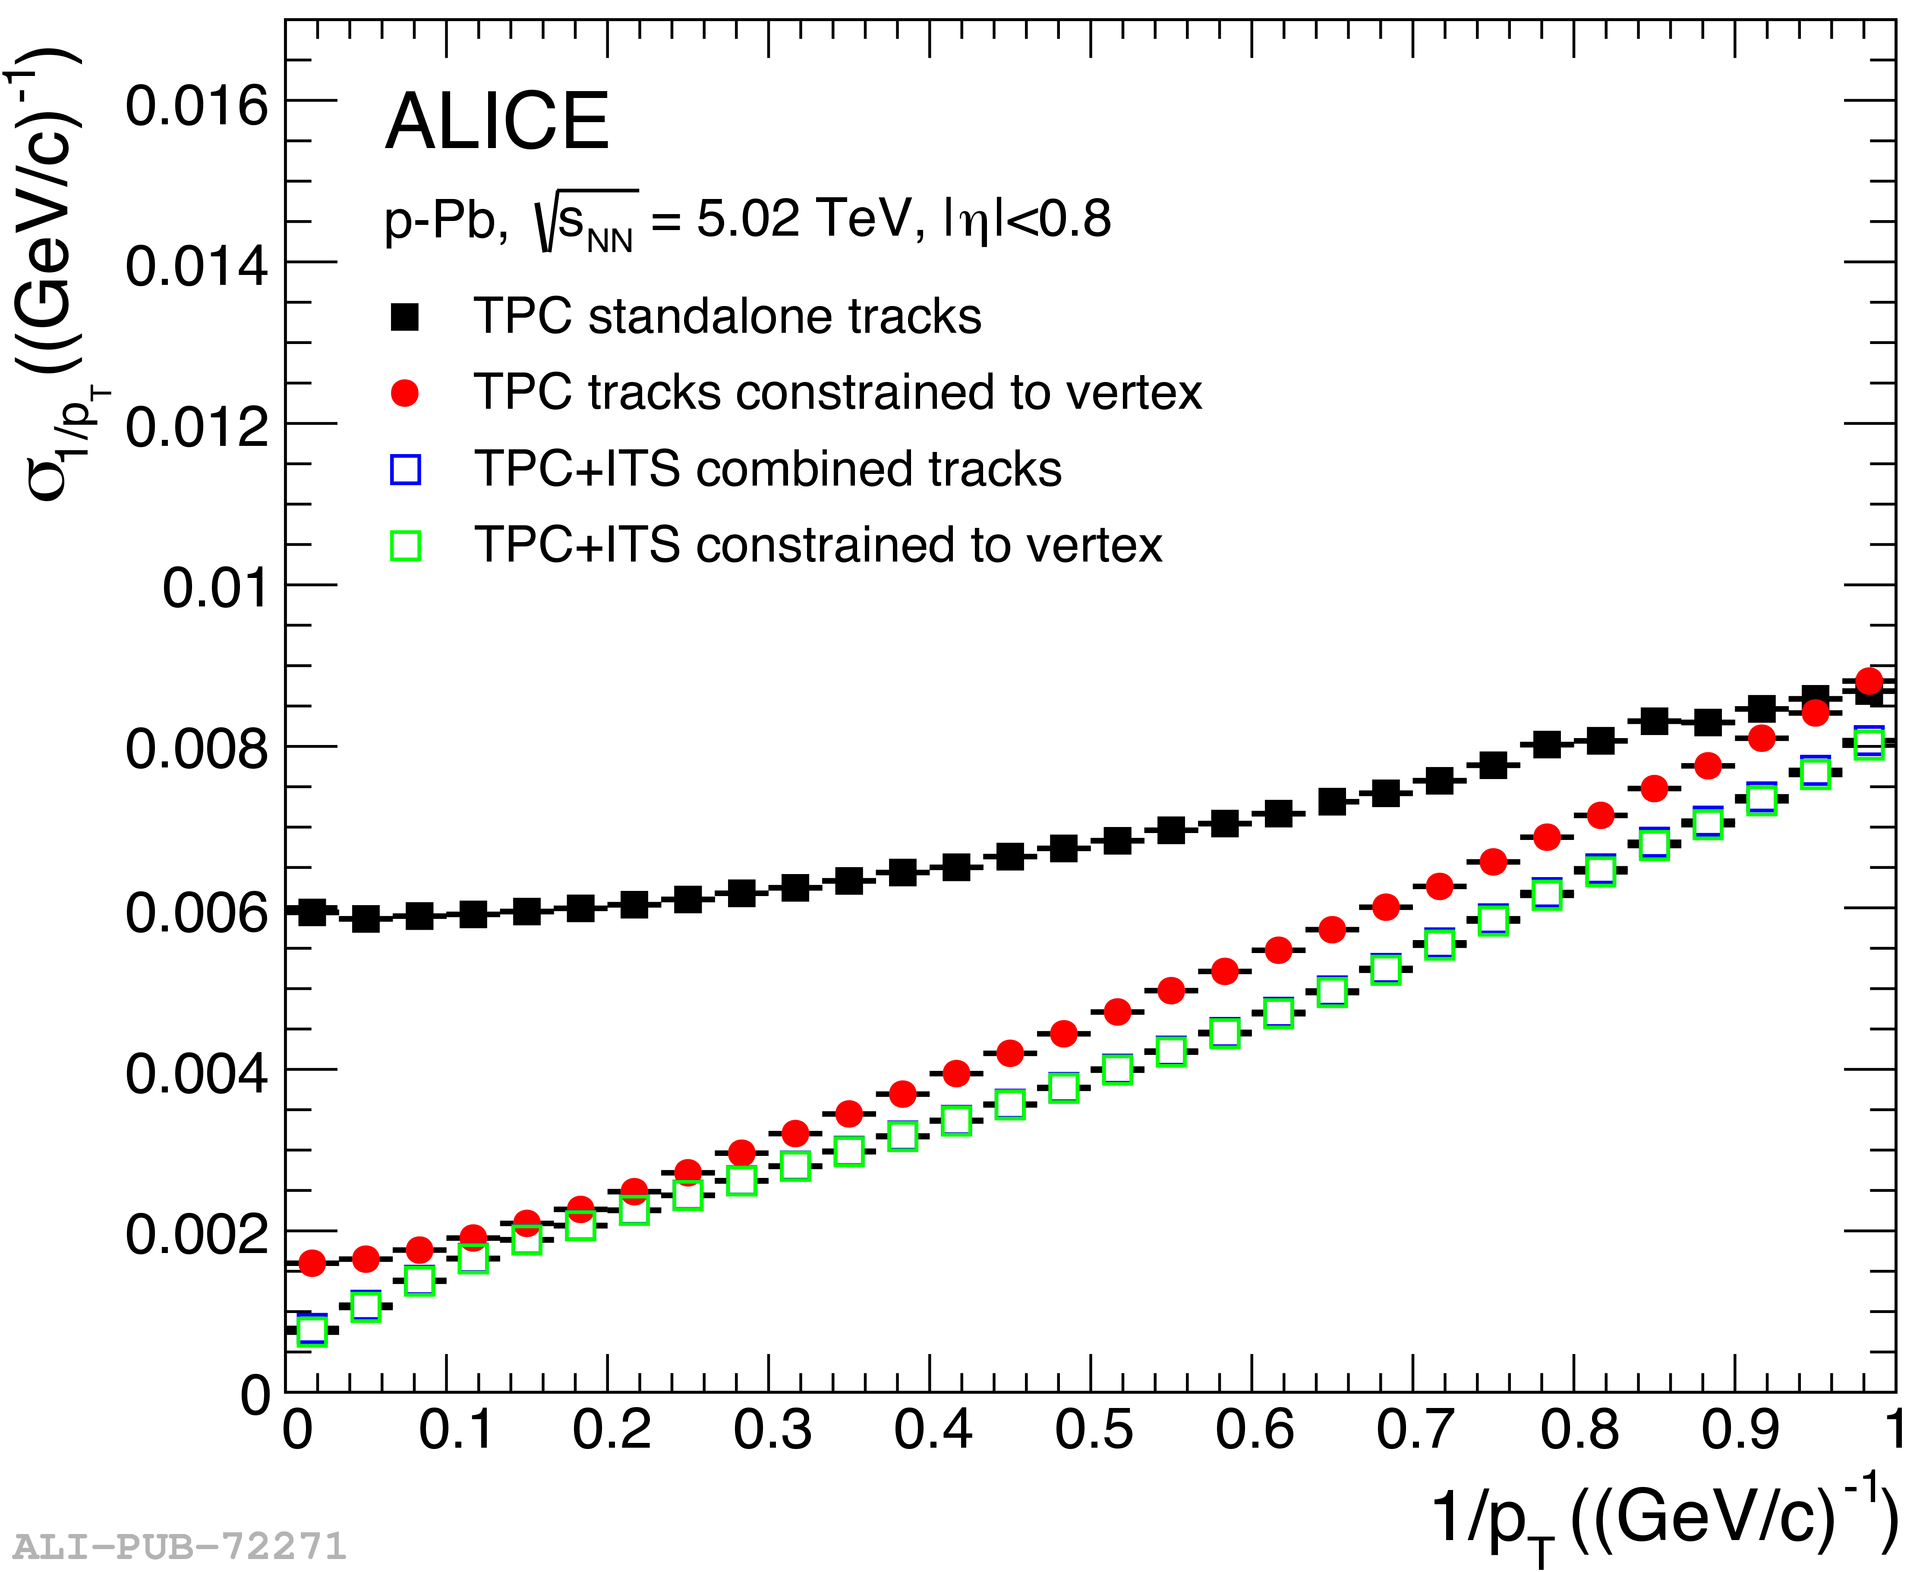
\includegraphics[width=0.6\textwidth]{gfx/ptresolution}
	\caption{Resolution on the 1/\pt parameter as a function of 1/\pt in \pPb collisions at \sctev. The resolution is quoted for TPC tracks with (red dots) and without (black squares) vertex constraint and for ITS+TPC tracks with (green square) and without (blue square) vertex constraint. The resolution is quoted for 1/\pt because this can be extracted directly from the covariance matrix of the Kalman Filter fit.}
	\label{fig:vertres}
\end{figure}

Following the described process the ALICE apparatus can reconstruct track with resolution
between 1\% and 10\% in the momentum range from 0.1 to 100 \gevc. 
Figure~\ref{fig:vertres} shows the 1/\pt resolution for standalone TPC and ITS+TPC tracks which
is related to the \pt resolution by the formula:
\begin{equation}
    \frac{\sigma_{\pt}}{\pt} = \frac{\sigma_{1/\pt}}{1/\pt}.
\end{equation}
The effect of constraining the tracks to the primary vertex is shown as well and considering,
for instance, TPC standalone tracks the resolution is reduced from 6\% to 2\% at low \pt by applying
this requirement.

%
\subsection{Vertexing} \label{sec:vertexing}

\subsubsection{Primary vertex reconstruction}
A first estimation of the interaction vertex is obtained by using the clusters on the two layers of 
SPD. The algorithm matches the clusters on the SPD layers inside a fixed azimuthal window,
building a set of segments, called tracklets.
Then the space point which minimises the distance from all the tracklets is computed and it corresponds to the estimation of
the interaction vertex.
At least two tracklets are required for a 3D reconstruction of the primary vertex position.
This estimation is very fast, but the most precise determination of the primary vertex position is 
obtained by using the full reconstructed track information (Fig.~\ref{fig:vertres}).
The full reconstructed tracks, obtained at the end of the tracking procedure, are propagated to the
nominal beam line and the tracks too far from it are excluded from the vertex computation.

\begin{figure}
    \centering
    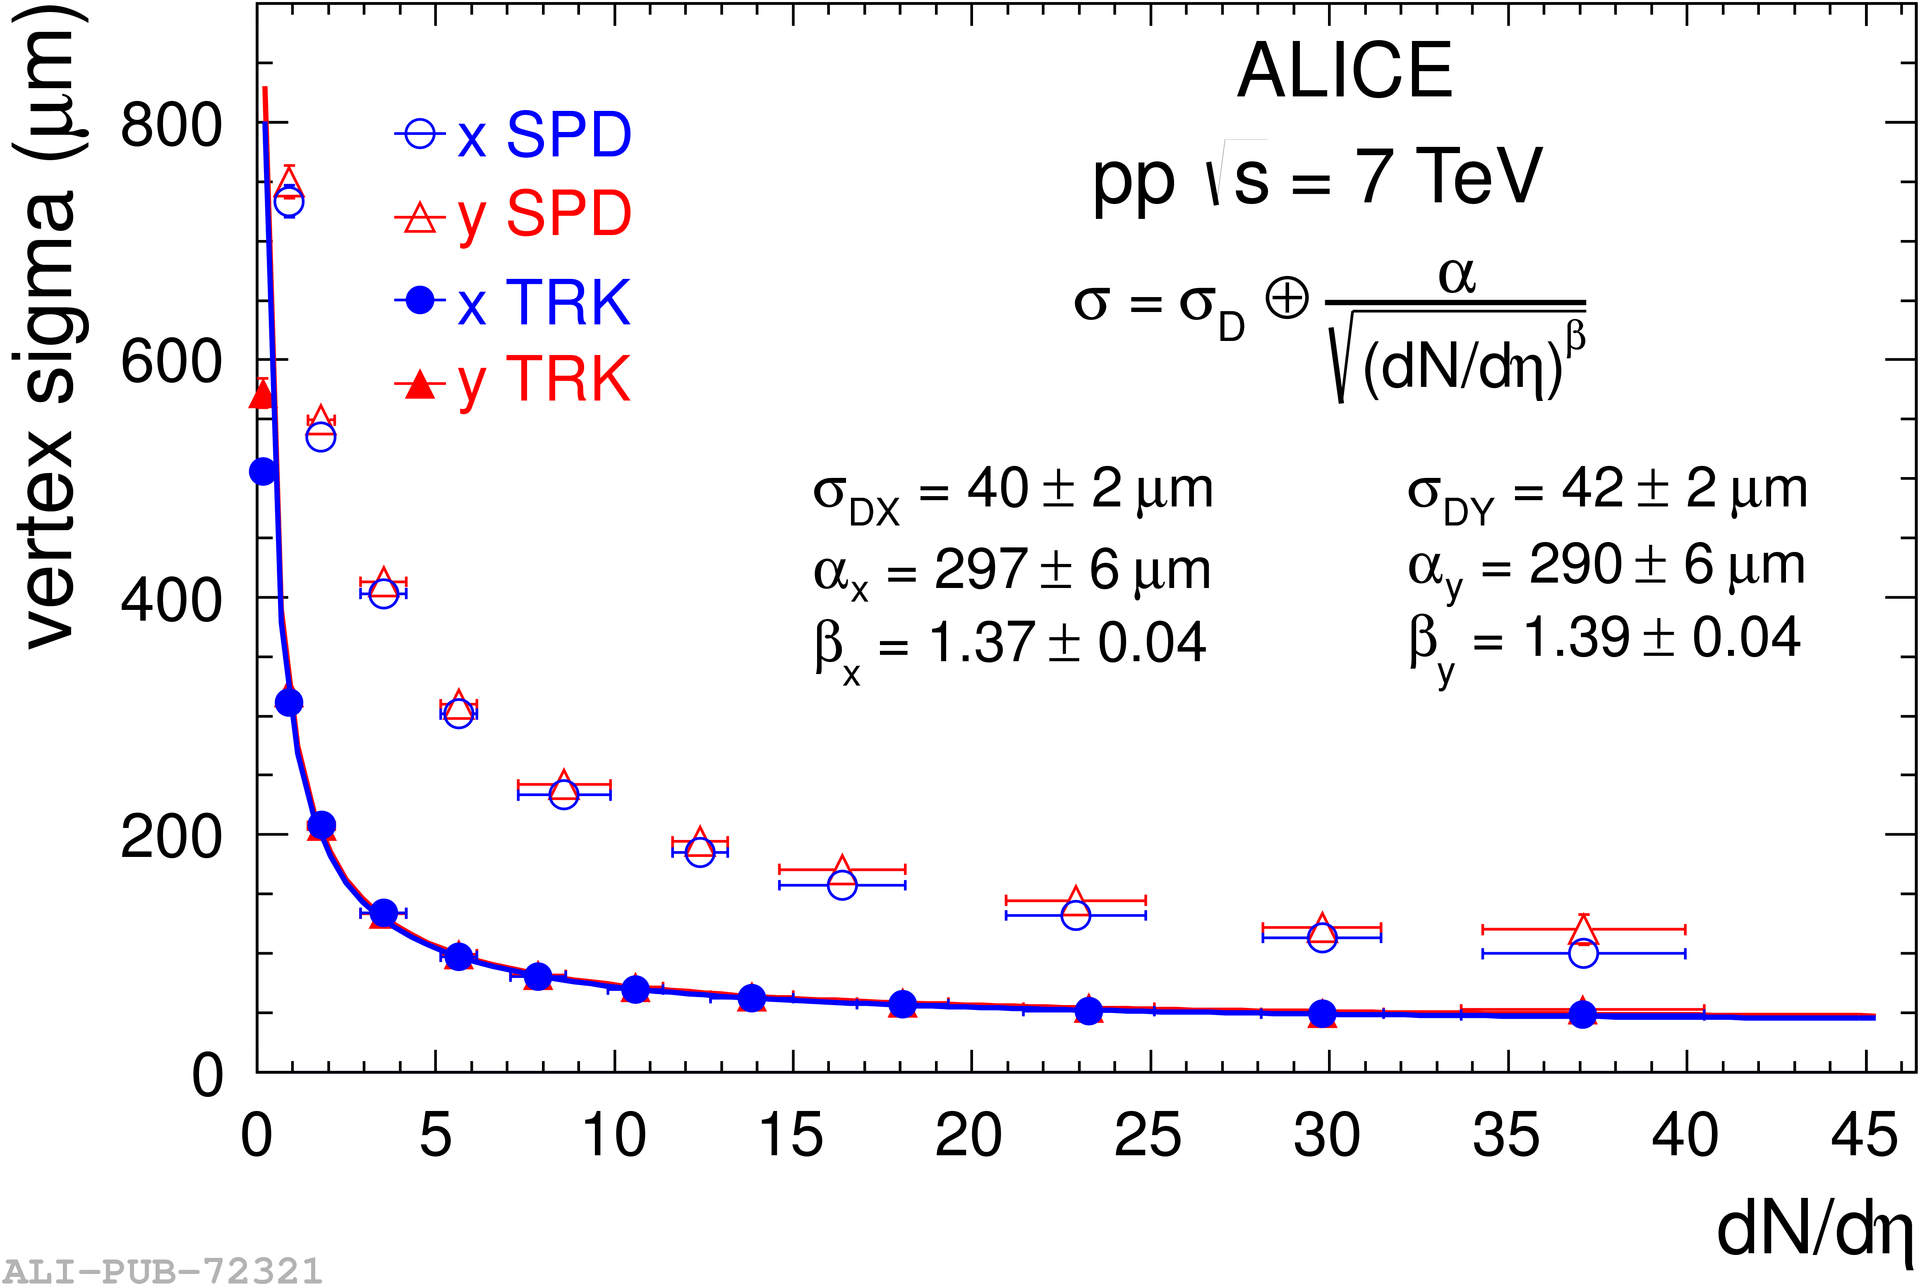
\includegraphics[width=0.7\textwidth]{gfx/vertexres}
	\caption{Resolution on the primary vertex position using the SPD clusters (open markers) and the full track informations (full markers) as a function of the charged particle multiplicity of the event in pp collisions at $\sqrt{s} = 7 \mathrm{TeV}$~\cite{alicemulti}.}
	\label{fig:vertres}
\end{figure}

\subsubsection{Secondary vertex reconstruction}
Once the tracks and the primary vertex have been reconstructed, the event reconstruction procedure
searches for secondary vertices from particle decays.
The reconstruction of the secondary vertices from decays of neutral particles and with a V-shaped 
track topology of the daughters is performed with the $V^{0}$ finder algorithm.
The basic principle of the $V^{0}$ finder algorithm is the matching of two tracks with opposite sign,
which are close in the space and presumably come from the decay of one mother particle.
The combined tracks and the resulting mother momentum are requested to pass quality and topology
selection criteria before being tagged as $V^{0}$ candidate.
The $V^{0}$ finder algorithm is implemented in the ALICE software and performed with two different
procedures, the offline $V^{0}$ and the on-the-fly $V^{0}$.

In the reconstruction process the Distance of Closest Approach (DCA) -- the minimum 
distance of the track from the reconstructed vertex -- is computed for all the reconstructed
track in the beam line direction (DCA$_{z}$) and in the transverse plane (DCA$_{xy}$).
These two parameters are stored together with the track to be then used in the offline data analyses
to reject tracks that do not come from the primary vertex.

%
\subsection{Particle Identification} \label{sec:PID}

One of the main feature of the ALICE experiment is the capability of performing a Particle
Identification with high resolution.
To achieve these performances the information provided by different detectors are combined.
For the charged hadron identification the ITS, the TPC, the TOF and the HMPID are used.
The ITS and the TPC provide information on the specific energy loss of the tracked charged particles.
The TOF detector measures the time of flight and the HMPID is a ring-imaging Cerenkov detector that
measures the Cerenkov angle to determine the $\beta = v / c\ $ of the particle.
Those detectors can be used all together but, usually, the particle identification is performed
combining the information provided by few of them.
The choice of the detectors to be used for the PID depends on the physics channel studied in a
particular analysis.

\subsubsection{TPC particle identification} \label{sec:TPC_PID}

\begin{figure} 
    \centering
    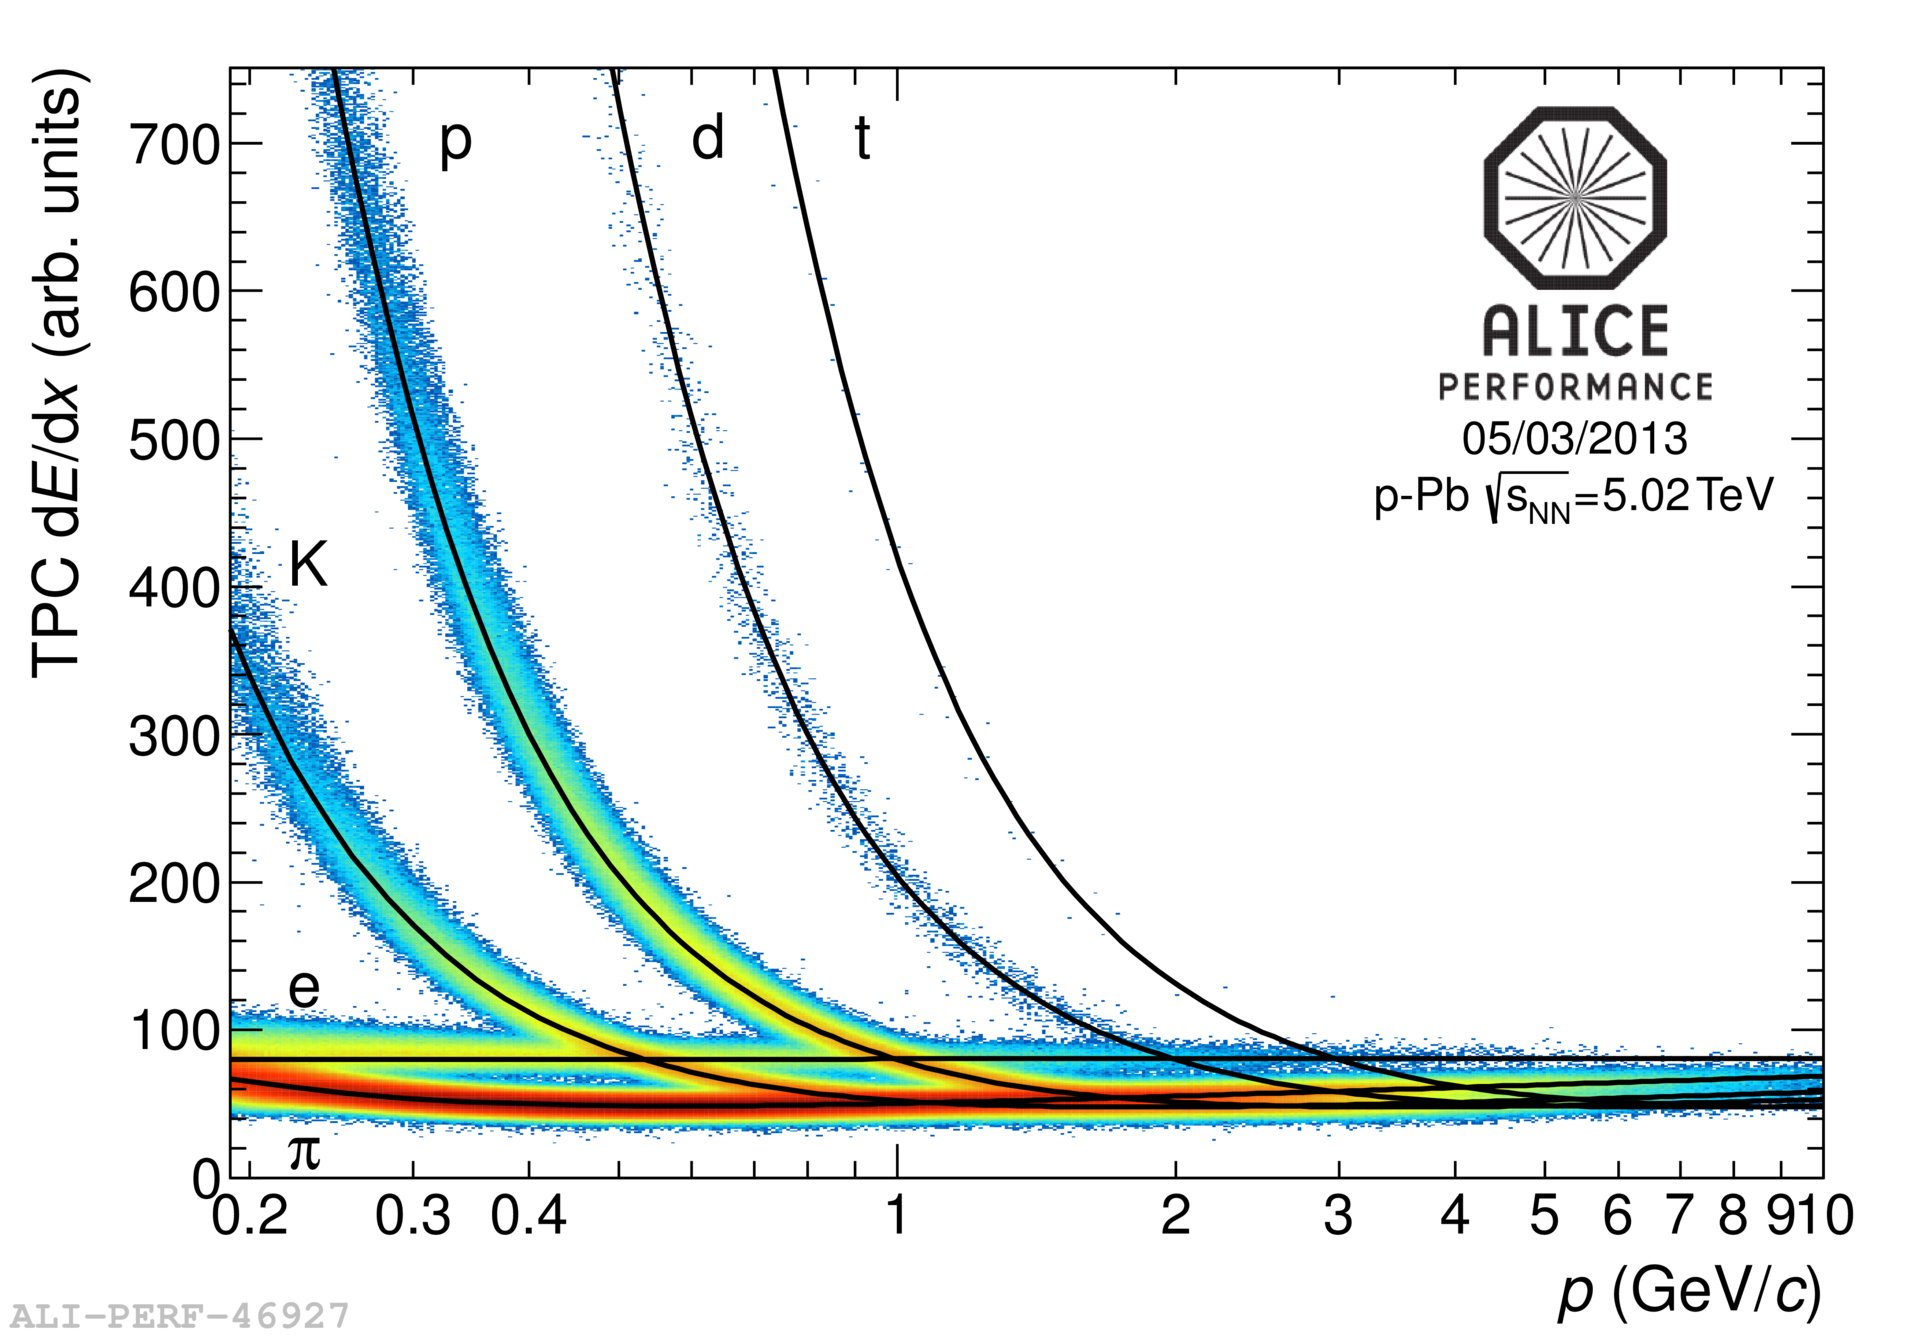
\includegraphics[width=0.75\textwidth]{gfx/pid_tpc_gen}
	\caption{Specific energy loss as a function of the rigidity for particles traversing the TPC gas in \pPb collisions at \sctev. The black lines represent the expected detector response for different particles.}
	\label{fig:pid_tpc}
\end{figure}

In the TPC particles are identified by measuring their specific energy loss in the detector gas.
Up to 159 padrows measure the charge generated in the gas by the passing particle by means of the
ionisation process. 
This charge is related to the particle energy loss by the value of the detector electric
field and by gain factors linked to the detector features. 
The resulting \dedx is obtained as the truncated mean of the single padrow measurement.

Particle identification is performed by measuring simultaneously the specific energy loss \dedx 
and the momentum of each particle traversing the detector gas.
The energy loss as a function of the momentum in TPC has been parametrised with a function originally
proposed by the ALEPH collaboration~\cite{aleph}:
\begin{equation} \label{eq:aleph}
    f(\beta \gamma) = \frac{P_{1}}{\beta^{P_{4}}} \left( P_{2} - \beta^{P_{4}}
    - \ln \left( P_{3} + \frac{1}{(\beta \gamma)^{P_{5}}} \right) \right),
\end{equation} 
where $\beta$ is the particle velocity, $\gamma$ is the Lorentz factor and $P_{1-5}$ are the fit
parameters, obtained from a fit to the experimental data.
Alternatively the response functions have been parametrised using splines as shown in 
Figure~\ref{fig:pid_tpc} which are provided by the ALICE analysis framework.

Finally, particles are identified adopting the $n\sigma$ method.
This method consists in selecting a fiducial band around the expected signal \ -- \dede in the case of
the  particle identification with the TPC -- \ for the particle of interest.
For each track, the distance from the expected signal is computed in terms of 
number of $\sigma$, where $\sigma$ is the signal resolution obtained with a Gaussian fit to the 
\dedx distribution in different momentum intervals:
\begin{equation} \label{eq:nsigma}
    n\sigma = \frac{S_{measured} - S^{i}_{expected}}{\sigma^{i}_{expected}}.
\end{equation}
In Eq.~\ref{eq:nsigma} $S_{measured}$ is the measured signal for the candidate track,
$S^{i}_{expected}$ is the expected signal for the species $i$ and $\sigma^{i}_{expected}$ is the
expected detector resolution for the same species $i$.

In the specific case of the TPC particle identification $S^{i}_{expected}$ represents the
expected specific energy loss for the species $i$ \ -- given by the equation~\ref{eq:aleph}
or by the splines -- \ while $S_{measured}$ is the measured \dedx.

The \dedx resolution is about 5.2\% in pp collisions and 6\% in \PbPb collisions.
A clear identification of the particle species, with the TPC, is possible up to $p \sim 1 \gevc$,
since at higher momenta the specific energy loss of different particle species are superimposed.

\begin{figure} [!h]
    \centering
    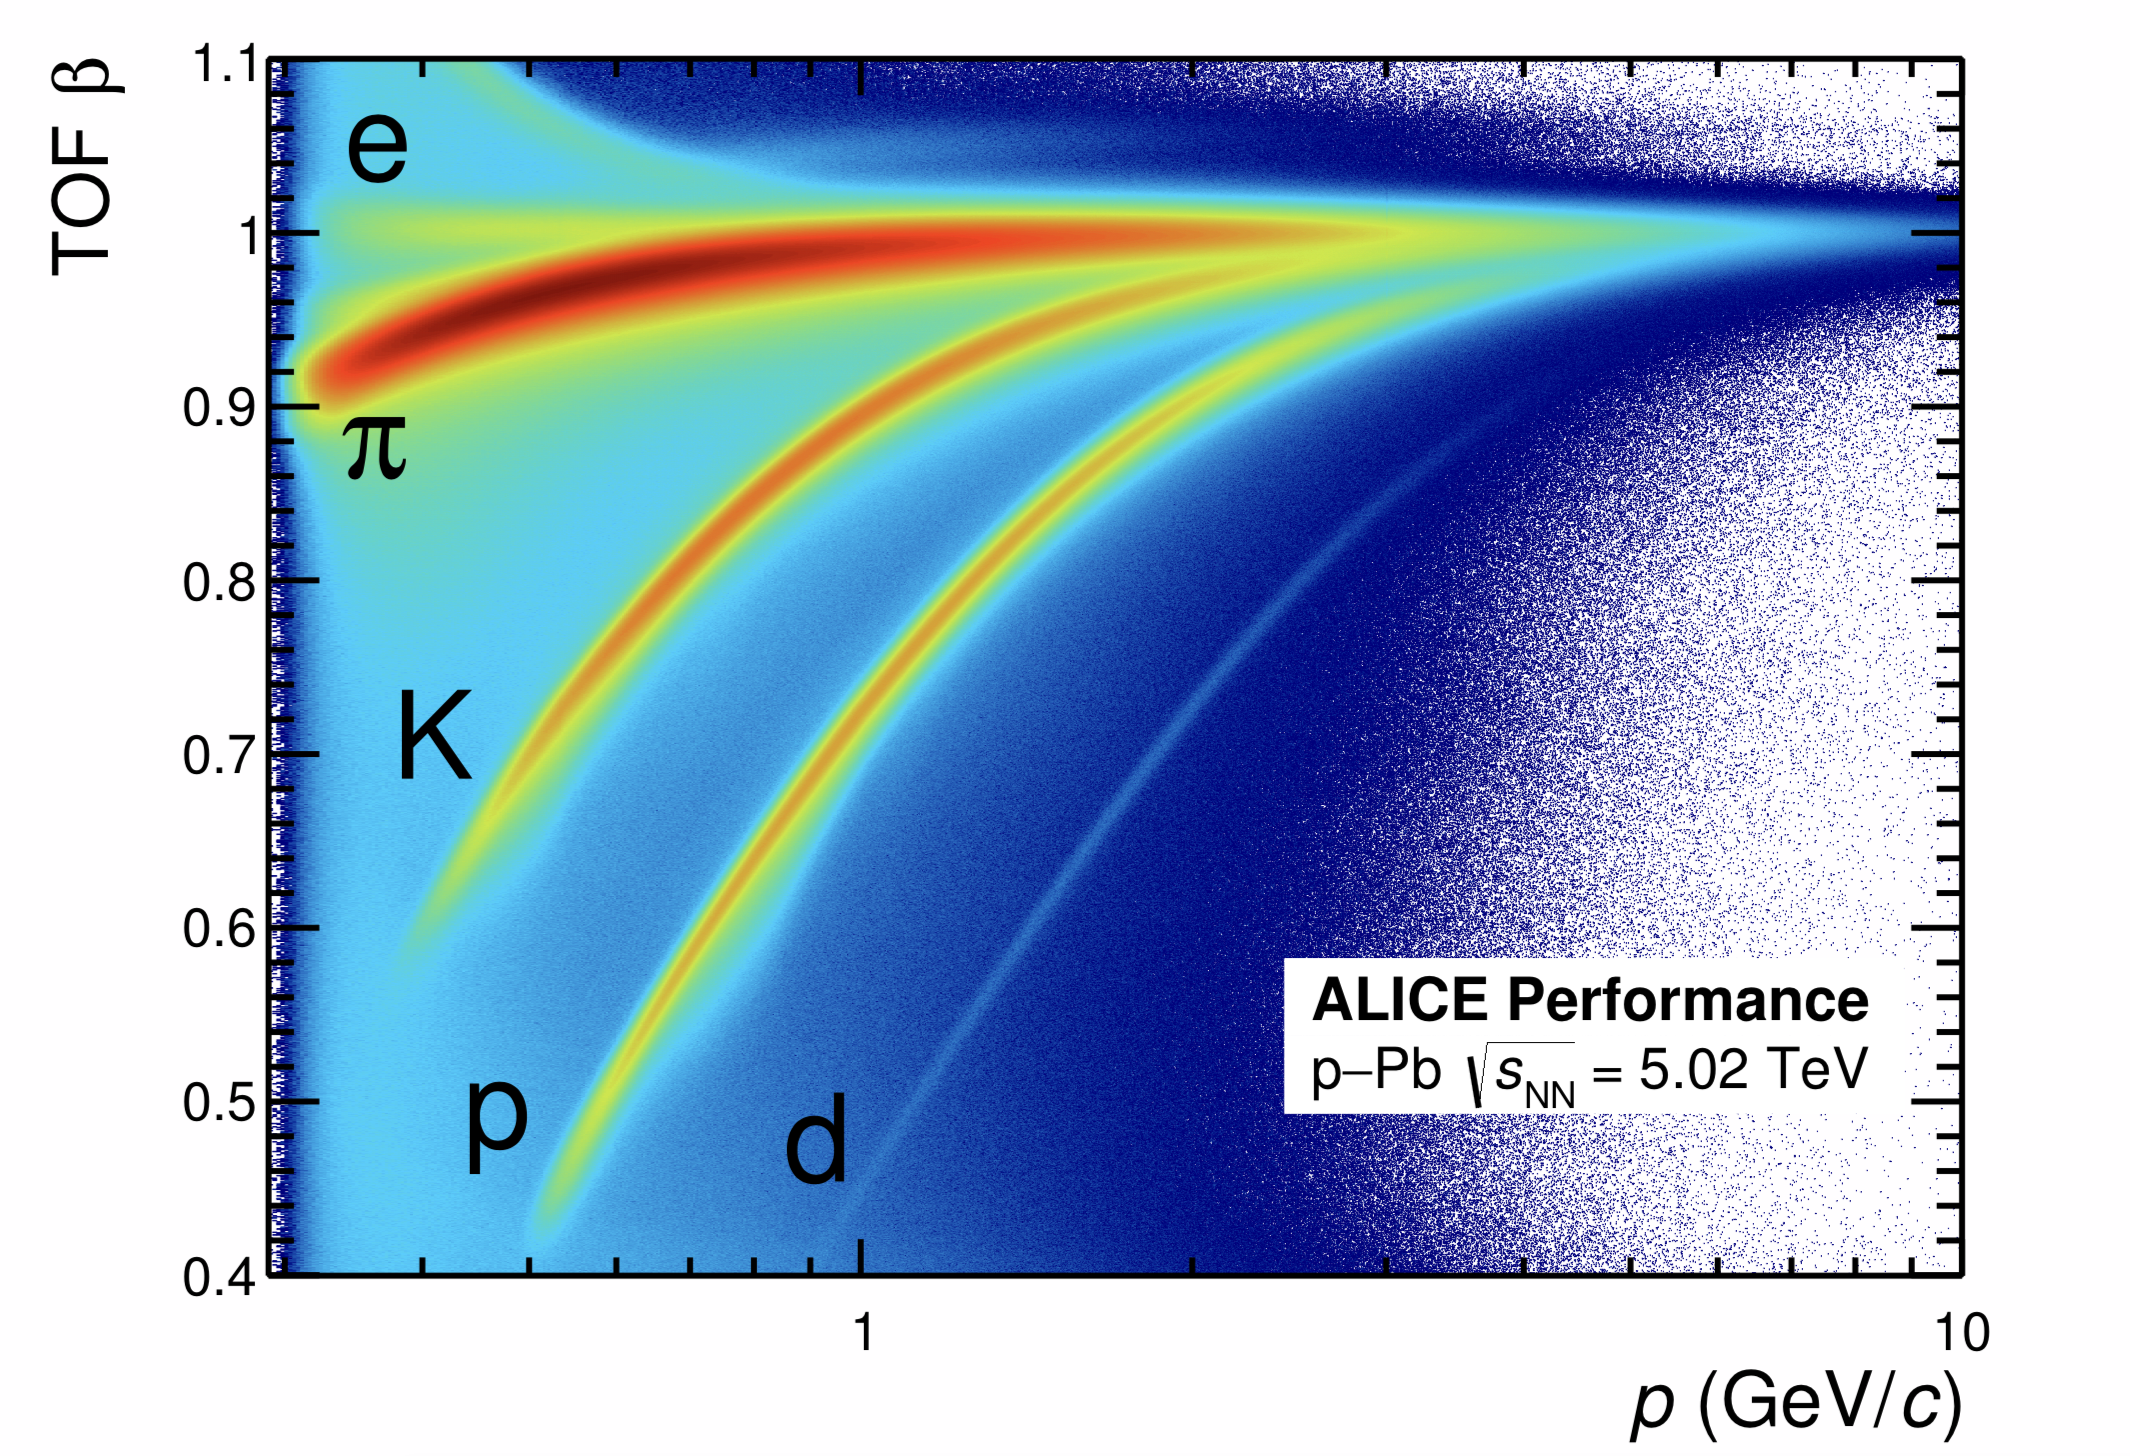
\includegraphics[width=0.75\textwidth]{gfx/pid_tof}
	\caption{$\beta$ of the particles in \pPb events at \sctev computed using the time of flight information from the TOF detector as a function of the measured track momentum.}
	\label{fig:pid_tof}
\end{figure}

\subsubsection{TOF particle identification} 

The TOF detector, described in Section~\ref{sec:tof}, is used to determine the mass of a particle by
measuring the time of flight.
As a matter of fact, the measured time of flight $t_{TOF}$ and the integrated track length $L$ are used
to compute in the tracking process the $\beta$ of the particle by adopting the classical formula:
\begin{equation}
    \beta\,c = \frac{t_{TOF}}{L}.
\end{equation}
Figure~\ref{fig:pid_tof} shows the measured particle $\beta$ as a function of the momentum estimated
in the tracking procedure.
It is also visible the mismatch background, which is due to tracks incorrectly matched to TOF
clusters. This background is an effect related to the TOF occupancy.

The particle identification with TOF detector is performed by using the $n\sigma$ method described in the 
previous section (Sec.~\ref{sec:TPC_PID}). In the specific case of the TOF, the measured and the 
expected signal are represented by the measured and the expected time of flight of a specific
particle specie.

Thanks to its excellent time resolution the TOF detector provides the information for PID in the
intermediate momentum range, up to 2.5 \gevc for pions and kaons, 4 \gevc for protons and 5 \gevc
for deuterons.
